% %%%%%%%%%%%%%%%%%%%%%%%%%%%%%%%%%%%%%%%%%%%%%%%%%%%%%%%%%%%%%%%%%%%%%%
% Dummy Chapter:
% %%%%%%%%%%%%%%%%%%%%%%%%%%%%%%%%%%%%%%%%%%%%%%%%%%%%%%%%%%%%%%%%%%%%%%

% %%%%%%%%%%%%%%%%%%%%%%%%%%%%%%%%%%%%%%%%%%%%%%%%%%%%%%%%%%%%%%%%%%%%%%
% The Introduction:
% %%%%%%%%%%%%%%%%%%%%%%%%%%%%%%%%%%%%%%%%%%%%%%%%%%%%%%%%%%%%%%%%%%%%%%
\fancychapter{Numerical Discretization}
\label{cap:chapter-numerical}

\textit{In this chapter the discretization methods are introduced and discussed, followed by a proposal for the discretization for the previously presented conceptual models. Competing formulations may be introduced in order to further justify a specific choice or drive a given idea. Continuous interpolation theory is explored, introducing interpolating kernels. Discrete interpolation is described and analyzed, with discrete differential operators being derived. The \ac{DEM} method is introduced and expanded within the \ac{SPH} framework. A time integration scheme is introduced and discussed briefly, as well as the corresponding stability region.}

\section{Integral Interpolation and the SPH Method}
\label{sec:SPH}

\subsection{Introduction}

In \ac{SPH} an approximate numerical solution is obtained by expressing the continuous media by a set of interpolation points from which to compute the quantities being conserved. These points represent material particles, since the Lagrangian description implies that they move with the flow, 'carrying' a given mass. This perspective into the fundamental idea of the method justifies the \emph{particle} term being applied, in the sense of a numerical mass lump, a macroscopic \emph{quanta} of the discretized medium. 

The method was introduced by \cite{Gingold-1977} and simultaneously by \cite{Lucy-1977}, initially to solve astrophysical problems where Eulerian mesh-based methods were insufficient. As a purely Lagrangian, meshless scheme, \ac{SPH} poses a number of advantages over mesh-based methods. Advection is treated explicitly, since particles carry their properties with them. Motion of the media maps directly as motion of the \ac{SPH} particles. This provides an important advantage for multi-phase problems, as each particle can be assigned to a different phase. Similarly, interfacial or free-surface flows do not require the explicit tracking of the interface or free-surface of interest, as it will be implicitly defined by the positions of the particles. Unlike mesh-based methods, there is no topological connectivity\footnote{Topological connectivity is employed in the context of a numerical discretization exclusively, meaning a fixed list of neighbors with whom to interact does not exist in \ac{SPH}.} between traditional \ac{SPH} particles, as they interact with all of the neighbors according to their radial separation, mediated by an interpolating kernel function. This has profound implications, as many of the issues with generation and evolution of a complex, time-varying mesh are bypassed. Problems involving complex, moving geometry, elastic solids or the fracture of brittle solids are significantly simpler to treat using Lagrangian meshless methods.

Disadvantages of the approach include mostly accuracy and stability concerns, due to their difficult formal description. \ac{SPH} particles are not constrained to stay in a well-ordered, stable configuration. In a regular lattice traditional techniques for stability analysis and convergence studies are well known; in a purely random sampling, as a Monte Carlo method, these qualities are also simple to compute, at least approximately. In \ac{SPH} however, any lattice deforms, not randomly, but according to the conservation equations being solved, introducing an unexpected difficulty in analyzing the method under normal conditions. If on one hand, by respecting the conservation equations, the particles tend to keep evenly spaced, the instantaneous dynamics of the medium can cause the particles to become locally disordered.  \cite{Monaghan-2005} presents an analysis of the interpolation errors that occur for a 1D equi-spaced line of \ac{SPH} particles. \cite{Swegle-1995} and \cite{Morris-1997} performed a stability analysis of \ac{SPH}, providing results for 1D and 2D regular grids of particles. In contrast, there is much less information available on \ac{SPH} errors and instabilities for disordered particles \citep{Ellero-2011}. \cite{Monaghan-2005} and \cite{Dehnen-2012} calculated an upper bound on the errors due to a randomly distributed set of particles, corresponding to a Monte Carlo simulation. Both noted that the distributions resulting from \ac{SPH} simulations are significantly more ordered than pure random positions, hence with higher accuracy than traditional Monte Carlo methods, as \cite{Quinlan-al-2006} explored by attempting to actually derive an error estimate for a generic SPH particle distribution. Even if second order seems to be the limit for traditional \ac{SPH} models \citep{Monaghan-2005, Oger-al-2007}, satisfactory results are achieved due to their inherent conservation properties, that coupled with the other advantages, seem to provide a uniquely useful tool.

%%%%%%%%%%%%%%%%%%%%%%%%%%%%%%%%%%%%%%%%%%%%%%%%%%%%%%%%%%%%%%%%%%%%%%%%%%%%%%%%%%%%%%%%%%
\subsection{Continuous Interpolation}
\label{Subsec:Interpolation}

Consider a scalar field A, expressed as a spatial convolution product with the Dirac Delta function $\delta$

%
\begin{equation} \label{eq:interpolant_1}
A\left( {\ve{r}} \right) = \int_\Omega  {A\left( {{\ve{r}}'} \right)\; \delta \left( {{\ve{r}} - {\ve{r}}'} \right)d{{r}}'},
\end{equation}
%
where $\Omega$ denotes the domain corresponding to the continuous medium. The nature of the Dirac Delta function renders \eqref{eq:interpolant_1} computationally inadequate, forcing its approximation by a suitable weight function $W\left( {{\ve{r}} - {\ve{r}}'} \right)$, called an interpolation kernel, which is a regular function and defines a compact support region\footnote{A function is said to have compact support if it is zero outside of a compact set. In the context of this work, the compact support region is therefore defined as the $\ve{r}$ centered region for which the kernel function $W$ is not zero.}. With $\Omega'$ being the domain centered in $\ve{r}$, one can write

% 
\begin{equation} \label{eq:interpolant_2}
A\left( {\ve{r}} \right) \approx  \left\langle {A} \right\rangle \left( {\ve{r}} \right) = \int_{\Omega '}  {A\left( {\ve{r}'} \right)\; W \left( {{\ve{r}} - {\ve{r}}'} \right)d{{r}}'},
\end{equation}
%
with $\left\langle {A} \right\rangle \left( {\ve{r}} \right)$ defining an interpolated field. Expanding field $A$ as a Taylor series around point $\ve{r}$ and writing $\bar{\ve{r}}=\ve{r}-\ve{r}'$

% 
\begin{equation} \label{eq:interpolant_taylor_1}
A\left( {\ve{r}'} \right) = A\left( {\ve{r}} \right) - \frac{\partial A}{\partial \ve{r}}\cdot \bar{\ve{r}} + \frac{1}{2}\bar{\ve{r}}^T \frac{\partial^2 A}{\partial \ve{r}^T \partial \ve{r}} \bar{\ve{r}} + O\left( |\bar{\ve{r}}|^3 \right)
\end{equation}
%
Replacing \eqref{eq:interpolant_taylor_1} back to \eqref{eq:interpolant_2}
% 
\begin{equation} \label{eq:interpolant_taylor_2}
\begin{split}
\left\langle {A} \right\rangle \left( {\ve{r}} \right) = A\left( {\ve{r}} \right) \int_{\Omega_0} {W \left( {\bar{\ve{r}}} \right)d{{r}}'} - \frac{\partial A}{\partial \ve{r}} \cdot \int_{\Omega_0} {\bar{\ve{r}} W \left( {\bar{\ve{r}}} \right)d{{r}}'} \; + \\ +\; \frac{1}{2} \text{tr}\left(\frac{\partial^2 A}{\partial \ve{r}^T \partial \ve{r}}\right) \cdot \int_{\Omega_0} {\bar{\ve{r}} \times \bar{\ve{r}} W \left( {\bar{\ve{r}}} \right)d{{r}}'} + \int_{\Omega_0} {O\left( |\bar{\ve{r}}|^3 \right) W \left( {\bar{\ve{r}}} \right)d{{r}}'}
\end{split}
\end{equation}
%
where $\Omega_0$ is $\Omega'$ translated to the origin. Noting that in such conditions $d{{r}'}=d\bar{{r}}$, for the approximation $\left\langle {A} \right\rangle \approx A$ to be accurate up to first order, then

% 
\begin{equation} \label{eq:kernel_cond_1}
\int_{\Omega_0} {W \left( \bar{{\ve{r}}} \right)d{{r}}'}=1
\end{equation}
%
and

% 
\begin{equation} \label{eq:kernel_cond_2}
\int_{\Omega_0} {W \left( \bar{{\ve{r}}} \right)\bar{\ve{r}}d{{r}}'}=0
\end{equation}
%

Condition \eqref{eq:kernel_cond_1} implies that the kernel zeroth-order moment should be equal to one, similarly to the Dirac delta distribution. Condition \eqref{eq:kernel_cond_2} asks that the kernel first order moment should be zero. By construction, $\Omega_0$ is centrally symmetric\footnote{A centrally symmetric object in Euclidean space is invariant under point reflection through its center.} and for an even kernel 

% 
\begin{equation} \label{eq:kernel_cond_3}
W \left( -\bar{{\ve{r}}}\right) =W \left( \bar{{\ve{r}}}\right)
\end{equation}
%
and
% 
\begin{equation} \label{eq:kernel_cond_4}
\nabla W \left( -\bar{{\ve{r}}}\right) =-\nabla W \left( \bar{{\ve{r}}}\right)
\end{equation}
%

Making a variable change $\bar{{\ve{r}}}'=-\bar{{\ve{r}}}$, one can write condition \eqref{eq:kernel_cond_2} as

% 
\begin{equation} \label{eq:kernel_cond_5}
\int_{\Omega_0} {W \left( \bar{{\ve{r}}} \right) \bar{\ve{r}} d\bar{\ve{r}}} = \int_{\Omega_0} {W \left( -\bar{{\ve{r}}} \right) \bar{\ve{r}} d\bar{\ve{r}}} = - \int_{\bar{\Omega}_0} {W \left( \bar{{\ve{r}}'} \right) \bar{\ve{r}'} d\bar{\ve{r}}'},
\end{equation}
%
where $\bar{\Omega}_0$ is the symmetric of $\Omega_0$. Assuming symmetrical invariance ($\bar{\Omega}_0 = \Omega_0$), the integral must be equal to its opposite, true only if both integrals are null, rendering condition \eqref{eq:kernel_cond_2} satisfied. We can now reduce \eqref{eq:interpolant_taylor_2} to 

% 
\begin{equation} \label{eq:interpolant_taylor_3}
\left\langle {A} \right\rangle \left( {\ve{r}} \right) = A\left( {\ve{r}} \right) \;+\; O(h^2),
\end{equation}
%
where the integral giving the error is $O(h^2)$ because $W \left( \bar{{\ve{r}}'} \right) \bar{\ve{r}'} d\bar{\ve{r}}' \sim 1/h$. 

Applying approximation \eqref{eq:interpolant_2} to the field $\nabla A$ we may write

% 
\begin{equation} \label{eq:grad_kernel_1}
\begin{split}
\left\langle {\nabla A} \right\rangle \left( {\ve{r}} \right) = \int_{\Omega '} \frac{\partial A \left( {\ve{r}'} \right)}{\partial {\ve{r}}'} \; W \left( \bar{\ve{r}} \right)d{\ve{r}}'\;= \\
=\; \int_{\Omega '} \frac{\partial}{\partial {\ve{r}}'} \left( A \left( {\ve{r}'} \right)\; W \left( \bar{\ve{r}} \right)\right)d{\ve{r}}'\; -\; \int_{\Omega '} A \left( {\ve{r}'} \right) \; \frac{\partial W \left( \bar{\ve{r}} \right)}{\partial {\ve{r}}'}d{\ve{r}}'
\end{split}
\end{equation}
%
It is important to write the identity 

% 
\begin{equation} \label{eq:grad_kernel_2}
\frac{\partial W \left( \bar{\ve{r}} \right)}{\partial {\ve{r}}'}= - \frac{\partial W \left( \bar{\ve{r}} \right)}{\partial {\ve{r}}}
\end{equation}
%
Applying the Gauss theorem to the first integral and the identity to the second yields

% 
\begin{equation} \label{eq:grad_kernel_3}
\left\langle {\nabla A} \right\rangle \left( {\ve{r}} \right) = \oint_{\partial\Omega '} A \left( {\ve{r}'} \right) \; W \left( \bar{\ve{r}} \right) \ve{n}\left( {\ve{r}'} \right) d\Gamma\;+ \; \int_{\Omega '} A \left( {\ve{r}'} \right) \; \frac{\partial W \left( \bar{\ve{r}} \right)}{\partial {\ve{r}}}d{\ve{r}}',
\end{equation}
%
where $\ve{n}\left( {\ve{r}'} \right)$ is the normal unit vector to $\partial\Omega'$. Assuming that the kernel has compact support, the surface integral is reduced to $\partial \Omega \cap \Omega'$ (refer to Figure \ref{fig:cont_kernel}). In an infinite domain, or with a sufficiently distant point $\ve{r}$ from $\partial \Omega$, this boundary integral is zero and Equation \eqref{eq:grad_kernel_3} renders

% 
\begin{equation} \label{eq:grad_kernel_4}
\left\langle {\nabla A} \right\rangle \left( {\ve{r}} \right) = \; \int_{\Omega '} A \left( {\ve{r}'} \right) \; \nabla { W \left( \bar{\ve{r}} \right)}d{\ve{r}}',
\end{equation}
%
This defines a continuously interpolated gradient operator, identical to \eqref{eq:interpolant_2}, but using the kernel gradient as the interpolation function. This is equivalent to writing

\begin{equation} \label{eq:grad_kernel_5}
\nabla \left\langle {A} \right\rangle \left( {\ve{r}} \right) = \left\langle {\nabla A} \right\rangle \left( {\ve{r}} \right) \;+\; O(h^2),
\end{equation}
%
demonstrated by applying the gradient operator to \eqref{eq:interpolant_taylor_3}. Inserting \eqref{eq:interpolant_taylor_1} into \eqref{eq:grad_kernel_4} we may write

% 
\begin{equation} \label{eq:grad_kernel_6}
\begin{split}
\left\langle {\nabla A} \right\rangle \left( {\ve{r}} \right) = \; A \left( {\ve{r}} \right)\int_{\Omega '} \nabla { W \left( \bar{\ve{r}} \right)}d{\ve{r}}' \; -\; \frac{\partial A}{\partial {\ve{r}}}\cdot \left( \int_{\Omega '} \nabla { W \left( \bar{\ve{r}} \right) \times \bar{\ve{r}} }d{\ve{r}}' \right) \;+ \\
+\; \frac{1}{2} \frac{\partial^2 A}{\partial \ve{r}^T \partial \ve{r}} \cdot\left( \int_{\Omega '} \nabla { W \left( \bar{\ve{r}}\right) \times \bar{\ve{r}} \times \bar{\ve{r}} }d{\ve{r}}' \right) \; + \; O(h^2)
\end{split}
\end{equation}
%
In order to have second-order accuracy on $\nabla \left\langle {A} \right\rangle \left( {\ve{r}} \right) \approx \left\langle {\nabla A} \right\rangle \left( {\ve{r}} \right)$ the conditions are

% 
\begin{equation} \label{eq:grad_kernel_cond_1}
\begin{split}
\int_{\Omega_0} \nabla { W \left( \bar{\ve{r}} \right)}d\bar{\ve{r}} \;=\: 0 \\
\int_{\Omega_0} \nabla { W \left( \bar{\ve{r}} \right) \times \bar{\ve{r}} }d\bar{\ve{r}} \;=\; -\ve{I} \\
\int_{\Omega_0} \nabla { W \left( \bar{\ve{r}}\right) \times \bar{\ve{r}} \times \bar{\ve{r}} }d\bar{\ve{r}} \;=\; 0
\end{split}
\end{equation}
%
where $\ve{I}$ is the identity. The first and last conditions are inherently satisfied by \eqref{eq:kernel_cond_4}. The second condition requires some manipulation:

% 
\begin{equation} \label{eq:grad_kernel_cond_2}
\begin{split}
\int_{\Omega_0} \nabla { W \left( \bar{\ve{r}} \right) \times \bar{\ve{r}} }d\bar{\ve{r}} = \int_{\Omega_0} \left[ \frac{\partial}{\partial \bar{\ve{r}}} \left( W \left( \bar{\ve{r}} \right)  \bar{\ve{r}} \right) - W \left( \bar{\ve{r}} \right) \left( \frac{\partial\bar{\ve{r}}}{\partial\bar{\ve{r}}} \right)^T  \right] d\bar{\ve{r}} \;=\\
=\; \oint_{\partial\Omega_0} W \left( \bar{\ve{r}} \right)\bar{\ve{r}} \times \ve{n}\left( \bar{\ve{r}} \right) d\Gamma\; -\; \left( \int_{\Omega_0} W \left( \bar{\ve{r}} \right) d\bar{\ve{r}}  \right)\ve{I}
\end{split}
\end{equation}
%
The surface integral is zero in the domain and property \eqref{eq:kernel_cond_1} renders the second condition of \eqref{eq:grad_kernel_cond_1} true.

A note should be made on a crucial assumption on these demonstrations, regarding a typical concern on interpolation methods: the boundaries. Conditions \eqref{eq:kernel_cond_1}, \eqref{eq:kernel_cond_2} and \eqref{eq:grad_kernel_cond_1} are true assuming that the compact support kernel $W \left( \bar{\ve{r}} \right) $ has no intersection with the boundary of the domain, \textit{i.e.} $\partial \Omega \cap \Omega' = 0$. Figure \ref{fig:cont_kernel} illustrates an intersection of $\partial \Omega $ and $\Omega'$.

%
\begin{figure}[ht!]
	\centering 
	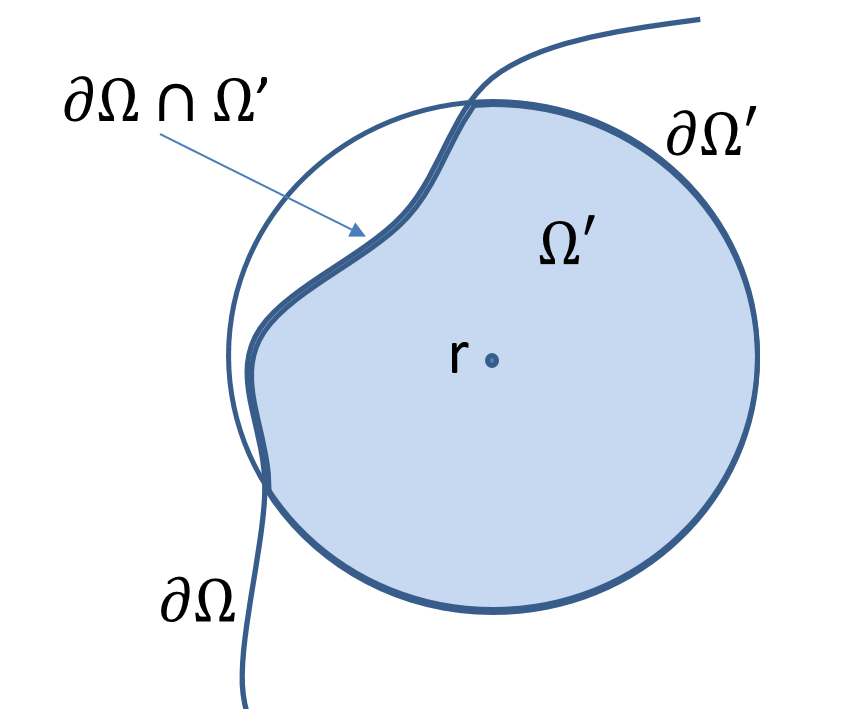
\includegraphics[width=0.30\linewidth]{Figures/3.Chapter/cont_kernel}
	\caption{Compact support kernel and domain boundary.}
	\label{fig:cont_kernel} 
\end{figure}
%
In this case the kernel zeroth-order momentum would not be one, deviating from the Dirac delta distribution and we would not be able to ensure first order consistency for the kernel approximation. Surface integrals in expressions \eqref{eq:grad_kernel_3} and \eqref{eq:grad_kernel_cond_2} would not disappear, leading to a loss of gradient information near the boundary and also order consistency. These problems meet various mitigation strategies at the discrete level, treated in section \ref{Subsec:discrete_interp}.

%%%%%%%%%%%%%%%%%%%%%%%%%%%%%%%%%%%%%%%%%%%%%%%%%%%%%%%%%%%%%%%%%%%%%%%%%%%%%%%%%
\subsection{Kernels}
\label{Subsec:Kernels}

In order to ensure the qualities of the continuous interpolation derived in Section \ref{Subsec:Interpolation}, the kernels must define a compact support region and have defined derivatives. A vast body of literature has been dedicated to the subject of kernels, their properties and their performance in the context of an \ac{SPH} simulation. Apparently similar kernels can produce very different results \citep{Monaghan-2005, Macia-2011,Violeau-2012}, and it is an ongoing task to formally identify and quantify the characteristics that lead to such differences. For the purpose of this thesis, only two kernels are described, a $5^{th}$ order class 2 Wendland \citep{Wendland-1995} and a cubic spline kernel. Both can be written as 

% 
\begin{equation} \label{eq:Kernel_general}
	W(\ve{r},h)=\frac{1}{h^d}\tilde{W}(q)
\end{equation}
%
where $h$ is the smoothing length and defines the scale of the compact support radius for kernel, $d$ is the dimensionality and $q=|\ve{r}|/h$ is a non-dimensional distance.

For the Wendland kernel, the $5^{th}$ order class 2 radial interpolation function was reformulated to have a $2h$ radius compact support

% 
\begin{equation} \label{eq:Kernel_wendeland}
	\tilde{W}(q)=\alpha_d\left\{ {\begin{array}{*{20}{c}}
  {(1-\frac{q}{2})^4(1+2q)} \\\\
  0 
\end{array}} \right.
\;\;\;\;\
\begin{array}{*{20}{c}}
  \text{for}\;\;\;{0 \leq q \leq 2} \\\\
  \text{for}\;\;\;{q > 2} 
\end{array}
\end{equation}
%
where $\alpha_d$ takes values $\alpha_2=7/4\pi$ and $\alpha_3=21/16\pi$. 

The cubic spline kernel can be defined as 

% 
\begin{equation} \label{eq:Kernel_cubic}
	\tilde{W}(q)=\alpha_d\left\{ {\begin{array}{*{20}{c}}
  {1-\frac{3}{2}q^2+\frac{3}{4}q^3} \\\\
  {\frac{1}{4}(2-q)^3} \\\\
  0 
\end{array}} \right.
\;\;\;\;\
\begin{array}{*{20}{c}}
  \text{for}\;\;\;{0 \leq q \leq 1} \\\\
  \text{for}\;\;\;{1 \leq q \leq 2} \\\\
  \text{for}\;\;\;{q > 2} 
\end{array}
\end{equation}
%
where $\alpha_2=10/7\pi$ and $\alpha_3=1/\pi$. Figure \ref{fig:kernel_wendland} plots the kernels and respective first derivatives.

%
\begin{figure}[ht!]
	\centering 
	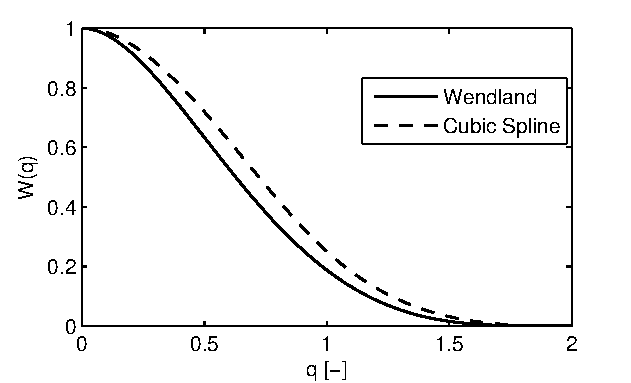
\includegraphics[width=0.49\linewidth]{Figures/3.Chapter/Kernels}
	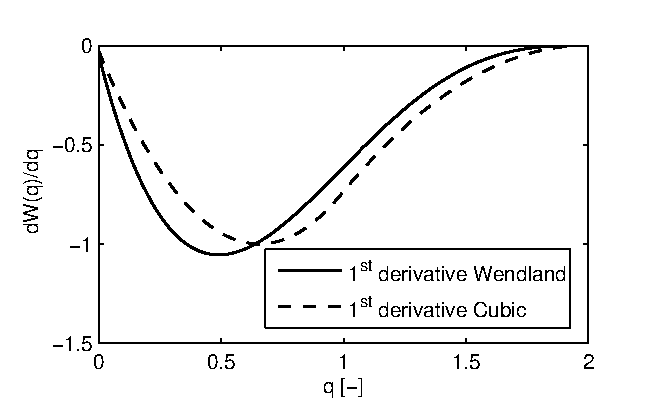
\includegraphics[width=0.49\linewidth]{Figures/3.Chapter/Kernels_deriv}
	\caption{Left - Wendland and Cubic spline kernels; Right - First derivatives.}
	\label{fig:kernel_wendland} 
\end{figure}
%
The kernels and the derivatives show very similar profiles, even tough they are one order apart. The cubic spline kernel is however known to cause tensile instability \cite{Monaghan-1999}, and requires corrections to definition \eqref{eq:Kernel_cubic}. According to \cite{Swegle-1995}, tensile instability seems to be directly related to the size of the region of the kernel where the second derivative is negative. Figure \ref{fig:kernel_wndland_d2} shows the second derivative of the considered kernels.

%
\begin{figure}[ht!]
	\centering 
	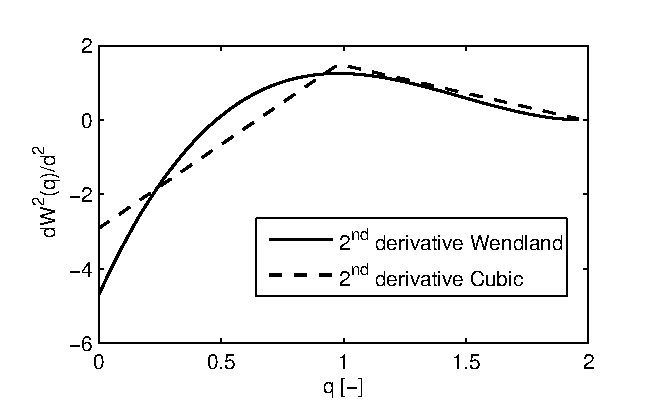
\includegraphics[width=0.49\linewidth]{Figures/3.Chapter/Kernels_2deriv}
	\caption{Second derivative of Wendland and Cubic spline kernels.}
	\label{fig:kernel_wndland_d2} 
\end{figure}
%
As can be noticed the size of these regions is similar, although the shape of the derivatives varies considerably. \cite{Macia-2011} performs an analysis of the performance of the Wendland kernel against a Gaussian kernel and finds that, even if apparently similar to the present comparison, the Wendland kernel out-performs other kernels considerably.


%%%%%%%%%%%%%%%%%%%%%%%%%%%%%%%%%%%%%%%%%%%%%%%%%%%%%%%%%%%%%%%%%%%%%%%%%%%%%%%%
\subsection{Discrete Interpolation}
\label{Subsec:discrete_interp}

As previously introduced, \ac{SPH} discretizes a continuous medium as a collection of Lagrangian interpolation nodes with mass. These points are called particles since they coincide with macroscopic material points that bear quantities such as velocity, density and position that change over time. Particle $i$ has a fixed mass of $m_i$, with volume $V_i$ and density $\rho_i$ related by

% 
\begin{equation} \label{eq:mass_volume_density}
V_i=\frac{m_i}{\rho_i}
\end{equation}
%
Assuming a reference density, a diameter $Dp$ can be set to compute the mass and reference volume of the particle.

In a strict Lagrangian framework, quantities of the particle will suffer a variation rate given by its Lagrangian derivative. For example, in the case of position and velocity

% 
\begin{equation} \label{eq:lagrang_posit}
\dot{\ve{r}}_i = \ve{v}_i = \frac{d\ve{r}_i}{dt}
\end{equation}
%
Expression \eqref{eq:lagrang_posit} contrasts with the Eulerian equivalent, since no advection terms are present, greatly simplifying the discretization.

The discretization of operators in \ac{SPH} is done by approximating the continuous integrals in section \ref{Subsec:Interpolation} by discrete summations. Employing a Riemann sum, one can write a scalar field as

% 
\begin{equation} \label{eq:discr_interp_1}
\left\langle {A} \right\rangle \left( {\ve{r}_i} \right) = \int_{\Omega '}  {A\left( {\ve{r}'} \right)\; W \left( {{\ve{r}_i} - {\ve{r}}', h} \right)d{{r}}'} \approx \sum_j{A_j V_j W(\ve{r}_{ij}, h)}
\end{equation}
%
The summation points are particle positions $\ve{r}_{j}$, where $A_j=A(\ve{r}_{j})$. $\ve{r}_{ij}$ represents $\ve{r}_{i}-\ve{r}_{j}$ and the volume of each $j$ particle accounts for the integration volume $d{\ve{r}}'$. Henceforth, without any loss of richness, the notation will be simplified: the subscripts $i$ and $j$ will tend to identify particles in the summation, $\ve{r}_{ij}$ will be used and it will be assumed that, dealing with a numerical approximation, the approximation notation will simply be represented by equality. The field is defined by the summation over all particles, but assuming compact support of the kernel this number is rendered finite. The sum is reduced to the particles inside the sphere of radius $\epsilon h$, as shown in Figure \ref{fig:kernel}

%
\begin{figure}[ht!]
	\centering 
	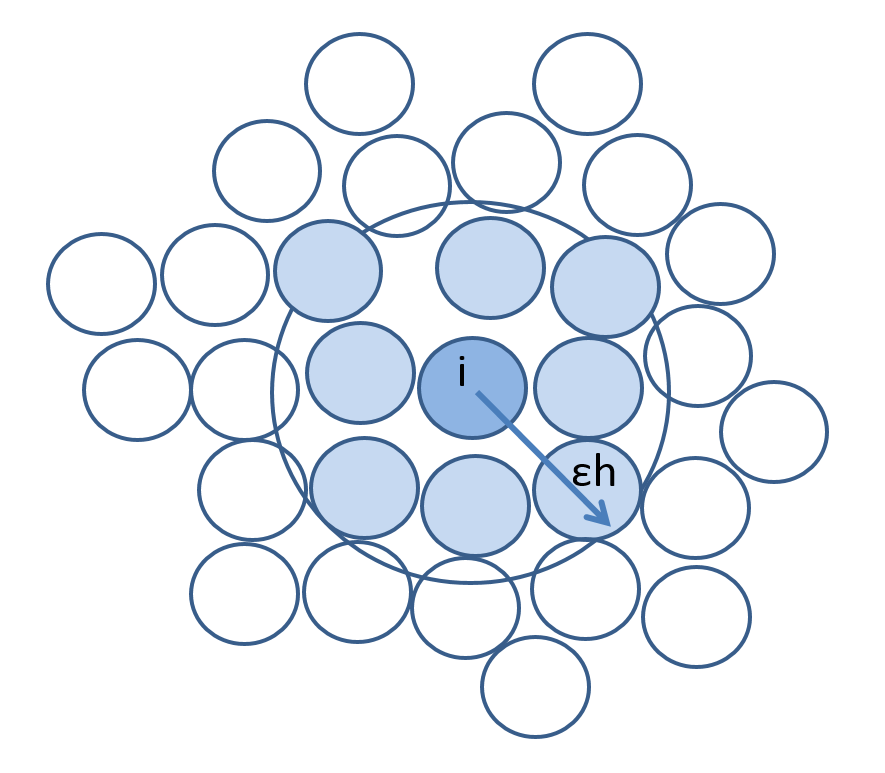
\includegraphics[width=0.40\linewidth]{Figures/3.Chapter/kernel}
	\caption{Summation extent for interpolation on particle $i$.}
	\label{fig:kernel} 
\end{figure}
%
In a 3 dimensions problem, the number of neighbors of a particle can range from a few tens to hundreds of points, summing an important disadvantage \ac{SPH} presents when compared with traditional, mesh-based methods: large computational cost.

Applying the discrete operator \eqref{eq:discr_interp_1} to vectorial quantities and notion \eqref{eq:grad_kernel_4} to differential operators we can write

% 
\begin{equation} \label{eq:discr_interp_2}
\begin{split}
A_i = \sum_j{A_j V_j W(\ve{r}_{ij}, h)} \\
\nabla {A}_i = \sum_j{A_j V_j \nabla W(\ve{r}_{ij}, h)} \\
\ve{A}_i = \sum_j{\ve{A}_j V_j W(\ve{r}_{ij}, h)} \\
\ve{\nabla} \cdot \ve{A}_i = \sum_j{ V_j \ve{A}_j \cdot \ve{\nabla} W(\ve{r}_{ij}, h)} 
\end{split}
\end{equation}
%

It should be noted that these expressions, although representing an exact derivative of the approximate function (considering no truncation effects on the kernel sampling), are written in a form that leads to a non zero derivative for a constant field. To ensure that gradients respect these properties one can write

% 
\begin{equation} \label{eq:discr_interp_3}
\nabla {A} = \frac{1}{\Phi}\left( \nabla(\Phi A)- A\nabla\Phi \right)
\end{equation}
%
where $\Phi$ is a differentiable function. In \ac{SPH} form

% 
\begin{equation} \label{eq:discr_interp_4}
\nabla {A}_i = \frac{1}{\Phi_i} \sum_j{\Phi_j V_j(A_j-A_i) \nabla W(\ve{r}_{ij}, h)}
\end{equation}
%
Equation \eqref{eq:discr_interp_4} returns a zero gradient for a constant field.  

Second derivatives can be estimated by differentiating an \ac{SPH} interpolant (Equation \eqref{eq:discr_interp_1}) twice:

% 
\begin{equation} \label{eq:2nd_der_sph_I}
\nabla^2 {A}_i  = \sum_j{A_j V_j \nabla^2 W(\ve{r}_{ij}, h)} 
\end{equation}
%
This expression, however elegant, presents a series of problems: i) it is very sensitive to particle disorder; ii) it is trivial to build a kernel whose second derivative changes sign on its defined region, possibly changing the sign of the second derivative independently of the behavior of the quantity, among other issues, properly explored by \cite{Brookshaw-1985, Monaghan-2005}. A more useful approach was proposed by \cite{Cleary-1996} and \cite{Morris-1997}

% 
\begin{equation} \label{eq:2nd_der_sph_II}
\nabla^2 {A}_i = \sum_j{A_j V_j \frac{\ve{r}_{ij}\cdot W(\ve{r}_{ij}, h)}{||\ve{r}_{ij}||^2}}
\end{equation}
%
This represents a hybrid combination of a finite difference derivative and a \ac{SPH} derivative. It has the advantage of bypassing the issues raised by taking a direct second derivative of the kernel function, at the expense of not fully conserving angular momentum \citep{Monaghan-2006}.


















\newpage
\section{Fluid discretization}
\label{sec:fluid-discretization}

This Section presents an attempt at discretizing Equations \eqref{eq:navier_cont} and \eqref{eq:navier_momentum}. With most particulate Lagrangian methods that is to say that the equations will be written with the corresponding discrete operators, in our case, the ones introduced in Section \ref{Subsec:discrete_interp}.

The continuity equation \eqref{eq:navier_cont} is traditionally discretized by employing the notion that $\rho \ve{\nabla} \cdot \ve{u} = \ve{\nabla} \cdot( \rho \ve{u}) - \ve{u} \cdot\ve{\nabla} \rho$, rendering equation \eqref{eq:navier_cont} as 
%
\begin{equation} \label{eq:sph_navier_cont}
	\frac{{d\rho_i }}{{dt}} = \sum_j{{m_j} \ve{u}_{ij} \cdot \ve{\nabla} W(\ve{r}_{ij}, h)}
\end{equation}
%
This is the equivalent of applying operator \eqref{eq:discr_interp_4} to approximate the $\ve{\nabla} \cdot \ve{u} $ field and taking $\Phi=\rho$. Equation \eqref{eq:sph_navier_cont} produces a zero divergence field for a constant $\ve{u}$ field. 

The approach of Sections \ref{Subsec:Interpolation} and \ref{Subsec:discrete_interp} was consistent with the designing of interpolation operators that would provide a desired accuracy. In particle methods, however, it becomes trivial and very tempting to interpret any equation in terms of pair-wise interaction between particles. For that purpose, we can agree that 

%
\begin{equation} \label{eq:physical_interp_I}
	\ve{\nabla} W(\ve{r}_{ij}, h) = \ve{r}_{ij}F(\ve{r}_{ij}, h)
\end{equation}
%
where $F(\ve{r}_{ij}, h) \leq 0$ is a function that respects Equation \eqref{eq:physical_interp_I}. The contribution of particle $j$ to the density variation of particle $i$ is then

%
\begin{equation} \label{eq:physical_interp_II}
	m_j\ve{u}_{ij} \cdot \ve{r}_{ij}F(\ve{r}_{ij}, h)
\end{equation}
%
This implies that approaching $ij$ particles i.e., for $\ve{u}_{ij} \cdot \ve{r}_{ij} \leq 0$, the interaction contributes with a positive density change, as our physical intuition expects. Equation \eqref{eq:sph_navier_cont} describes a medium that allows density changes, i.e., it is compressible. By allowing for \textit{some} compressibility the presented discretization is usually called \ac{WCSPH}. It has become the traditional \ac{SPH} way of modeling incompressible flows \citep{Monaghan-2005, Lee-2010}. Implementation is trivial since pressure is obtained from a \ac{EOS}, written so that the speed of sound is large enough to keep the relative density fluctuations small. \cite{Lee-2010} gives good insight into the relative accuracy of the pressure field of both \ac{WCSPH} and an incompressible approach, with the later being superior in most situations. Forcing incompressibility however, demands the solution of a large and potentially sparse Poisson problem at every time-step, built by defining a boundary at the free surface, that needs to be traced accurately. When dealing with highly distorted flows this is a major computational drawback and undermines the Lagrangian nature of the calculation. More details of the \ac{WCSPH} formulation are discussed in Section \ref{sec:eos}.

The pressure gradient of the Navier-Stokes equation (\eqref{eq:navier_momentum}) can be discretized in a number of ways. \cite{Gingold-1982} and \cite{Violeau-2012} used the discrete approximation of the Lagrangian of a particle system, using operators \eqref{eq:discr_interp_2} and \eqref{eq:discr_interp_4}. The same operators can be used directly to discretize the term in Equation \eqref{eq:navier_momentum}, leading to

%
 \begin{equation} \label{eq:sph_pressure_momentum}
\frac{\ve{\nabla}p_i}{\rho_i} = \sum_j{m_j \left( \frac{p_i}{\rho_i^2} +\frac{p_j}{\rho_j^2}\right) \ve{\nabla} W(\ve{r}_{ij}, h)},
\end{equation}
%
\noindent a symmetrical, balanced form of the pressure term that respects the action reaction principle. This implies that linear and angular momentum are conserved exactly by \eqref{eq:sph_pressure_momentum}. The second term of the second member in Equation \eqref{eq:navier_momentum} refers to the shear stresses, and it involves a second derivative of the velocity. As mentioned in Section \ref{Subsec:discrete_interp}, applying the SPH operators directly to the second derivative is avoided since it is too sensitive to particle disorder and limits the choice of the kernel functions. 

Three approaches to modeling this term are presented: the artificial viscosity model introduced by \cite{Gingold-1982}, the laminar viscosity model by introduced by \cite{Morris-1997} and the \ac{SPS} terms, properly presented in \cite{Dalrymple-2006} and discussed in Section \ref{sec:sps}.

\cite{Gingold-1982} introduced a momentum dissipating term in the form of a viscosity, designed to treat shock-tube problems. This form of numerical viscosity also mitigates problems due to instabilities arising in the system coming from the unstructured behavior of the particles, as well as accumulation of acoustic energy from integration errors during a simulation without dissipation. It is written as
%
\begin{equation}
\begin{split} 
\label{eq:sph_artificial_visc_I}
{
\ve{\Pi} _{i}} = \sum_j\left\{ {\begin{array}{*{20}{c}}
  {\frac{ \displaystyle { - \alpha {{\bar c}_{ij}}{\mu _{ij}}}}{\displaystyle {{{\bar \rho }_{ij}}}}\ve{\nabla}W(\ve{r}_{ij}, h)} \\ \\
  0 
\end{array}} \right.{\text{    }}\begin{array}{*{20}{c}}
  \text{if}\;\;\;{{{\ve{u}}_{ij}}\cdot{{\ve{r}}_{ij}} < 0} \\ \\
  \text{if}\;\;\;{{{\ve{u}}_{ij}}\cdot{{\ve{r}}_{ij}} \geqslant 0} 
\end{array} \;\;\; 
\hbox{with} \;\;\; {\mu _{ij}} = \frac{{({{\ve{u}}_{ij}}\cdot{{\ve{r}}_{ij}}}h)}{{{{r}}_{ij}^2}},
\end{split}
\end{equation}
%
\noindent where $c$ is the sound celerity and $\alpha$ is a parameter subject to calibration. This expression is traditionally used due to its simple implementation, conservation of linear and angular momentum and because it converges to $\mu {\ve{\nabla}^2}{\ve{u}}$ as $h \rightarrow 0$ \citep{Issa-2004}. It is however considered dissipative regarding shear and vorticity, and the case-dependent $\alpha$ parameter confirms its empirical nature.

\cite{Morris-1997}, influenced by the work of \cite{Cleary-1996}, proposed to model the shear viscosity by 

\begin{equation} \label{eq:sph_morris_laminar}
	\ve{\Pi}_{i} = \sum_j m_j \left( \frac{4\nu \ve{r_}{ij} \cdot \ve{\nabla}W(\ve{r}_{ij}, h) }{(\rho_i + \rho_j){{r}}_{ij}^2} \right)\ve{u}_{ij} 
\end{equation}
%
where $\nu$ is the actual kinematic viscosity of the fluid, defined as $\nu=\mu/\rho$. This expression conserves linear momentum but not angular momentum \citep{Colagrossi-2011}. Recent ideas over the local consistency of Expression \eqref{eq:sph_morris_laminar}, particularly in when the kernel is truncated, have been discussed by \cite{Colagrossi-2011} and \cite{Gonzalez-2009}.


The momentum equation (\eqref{eq:navier_momentum}) can now be written as
%\begin{equation} \label{eq:sph_navier_momentum}
%\begin{split}
%	\frac{{d{\boldsymbol{v}_i}}}{{dt}} = -\sum_j{m_j \left( \frac{p_i}{\rho_i^2} +\frac{p_j}{\rho_j^2} \right) \boldsymbol{\nabla} W(\boldsymbol{r}_{ij}, h)} +\\+ \sum_j m_j \left( \frac{4\mu \boldsymbol{r_{ij}} \boldsymbol{\nabla}W(\boldsymbol{r}_{ij}, h) }{(\rho_i + \rho_j)(|r_{ij}|^2 +\eta^2 )} \right)\boldsymbol{v}_{ij} + \sum_j{m_j \left( \frac{\tau_i}{\rho_i^2} +\frac{\tau_j}{\rho_j^2} \right) \boldsymbol{\nabla} W(\boldsymbol{r}_{ij}, h)} + {{\boldsymbol{g}}} 
%\end{split}
%\end{equation}
%%
\begin{equation} \label{eq:sph_navier_momentum_I}
	\frac{{d{\boldsymbol{u}_i}}}{{dt}} = -\sum_j{m_j \left( \frac{p_i}{\rho_i^2} +\frac{p_j}{\rho_j^2} \right) \boldsymbol{\nabla} W(\boldsymbol{r}_{ij}, h)} + \ve{\Pi}_{i} + \ve{g}
\end{equation}
%


%%%%%%%%%%%%%%%%%%%%%%%%%%%%%%%%%%%%%%%%%%%%%%%%%%%%%%%%%%%%
\subsection{Turbulence modeling}
\label{sec:sps}

Expressions \eqref{eq:sph_artificial_visc_I} and \eqref{eq:sph_morris_laminar} attempt to account for shear stresses developed at the scale of the interparticle interactions, $h$. Turbulent fluid flow however, may present very small local scales, depending on the Reynolds number, $R_e$ \citep{Batchelor-2000, pope-2000}. Attempting to model all of these scales is designated by \ac{DNS}, where no turbulent closures are needed. This imposes a serious limit on the range of possible $R_e$, since computational resources are limited. Opposite to this, the \ac{RANS} rely on closure models to estimate the stresses that arise even from large, energy-carrying structures. Another approach naturally compatible with our framework is to use \ac{LES} techniques, that can be understood as a intermediate between \ac{DNS} and \ac{RANS}. The idea is that the governing equations are spatially averaged over a length scale of the order of the numerical discretization. The contribution of the large structures to momentum and energy transfer is computed directly and only the effects of the smallest scales of turbulence are modeled. The hope is that, since the small scales tend to be more homogeneous and universal \citep{pope-2000}, the models can be simpler and require fewer adjustments when applied to different flows than similar models for the \ac{RANS}. 

To obtain the motion equations of the resolved scales, large and small scales must be separated. \ac{LES} is based on the definition of a filtering operation: a resolved variable is defined as

%
\begin{equation} \label{eq:eq_les_filter}
	\left\langle A \right\rangle(\ve{r})=\int_\Omega{A(\ve{r}')G\left( {{\ve{r}}, {\ve{r}}';\left\langle \Delta \right\rangle} \right)d{\ve{r}}'}  , 
\end{equation}
%
where $G$ is the filter function, the $\left\langle \; \right\rangle$ operator represents a generic spatial averaging and $\left\langle \Delta \right\rangle$ is the filter-width associated with the wavelength of the smallest scale retained by the filtering operation. Thus, the filter function determines the size and structure of the small scales. A special note should be given regarding the idea of the integral interpolant behind \ac{SPH} (Equation \eqref{eq:interpolant_1}) and the filtering operation of \ac{LES}. Since both \ac{SPH} and \ac{LES} share the same mathematical structure, it should come as no surprise that the combination of the methods seems very atractive to modelers.

\cite{Gotoh-2001} introduced this type of subgrid scaling for their incompressible \ac{MPS} method, as did \cite{Lo-2002} for their incompressible SPH method. For a compressible fluid, sub-particle scaling requires the use of special averaging, with Favre-averaging being the typically chosen in the literature. It is written as

%
\begin{equation} \label{eq:favre-average}
	\left\langle A \right\rangle=\frac{\left\langle\rho A\right\rangle}{\left\langle\rho\right\rangle}
\end{equation}
%
By using Favre-averaging, no new terms are introduced in the conservation equations, except for the \ac{SPS} terms. This means that Equations \eqref{eq:sph_navier_cont} and \eqref{eq:sph_navier_momentum_I} are implicitly in their filtered form, assuming $\left\langle A \right\rangle=A$\footnote{An acceptable abuse of notation since the averaged scale is indeed our working scale, no ambiguity is introduced.}. For the momentum Navier-Stokes equation, the application of a flat-top spatial filter yields \citep{Yoshizawa-1986} 

%
\begin{equation} \label{eq:navier_momentum_filtered}
		\frac{d\left\langle\ve{u}\right\rangle}{dt}= -\frac{1}{\left\langle\rho\right\rangle}\ve{\nabla}\left\langle p\right\rangle + \frac{1}{\left\langle\rho\right\rangle}\mu \ve{\nabla}^2\left\langle\ve{u}\right\rangle + \frac{1}{\left\langle\rho\right\rangle} \ve{\nabla}\cdot\ve{\tau}^* + \ve{g},
\end{equation}
%
where $\ve{\tau}^*$ is the \ac{SPS} tensor. Several proposals exist for the form of the tensor. Eddy-viscosity models try to reproduce the global exchange of energy between the resolved and unresolved stresses by mimicking the drain of energy associated with the turbulence energy cascade \citep{Batchelor-2000}. \cite{Yoshizawa-1986} proposed an eddy-viscosity model for weakly compressible turbulent flows using a multiscale direct-interaction approximation method. The anisotropic part of the \ac{SPS} is parametrized using the Smagorinsky (1963) model, while the \ac{SPS} energy is modeled by a  separate term

%
\begin{equation} \label{eq:sph_sps_visc}
	\frac{\ve{\tau}^*}{\left\langle\rho\right\rangle} = 2\nu_t \left( \left\langle\ve{D}\right\rangle - \frac{1}{3}\ve{\delta}\text{tr}\left(\left\langle\ve{D}\right\rangle\right) \right) - \frac{2}{3}C_I \Delta^2\ve{\delta}|\left\langle\ve{D}\right\rangle|^2,
\end{equation}
%
where $\nu_t=(C_S\Delta)^2|\left\langle\ve{D}\right\rangle|$ is the eddy viscosity, $C_S=0.1677$ is the Smagorinsky constant, $C_I=6.6\times10^{-3}$ and  $|\left\langle\ve{D}\right\rangle|=(2\left\langle\ve{D}\right\rangle\left\langle\ve{D}\right\rangle)^{1/2}$ \citep{Martin-al-2000}.

 
In \ac{SPH} notation, the \ac{SPS} term receives the same treatment as the pressure gradient term, in Equation \eqref{eq:sph_pressure_momentum}:

%
 \begin{equation} \label{eq:sph_sps_term}
\ve{\Pi}^{SPS}_{i} = \sum_j{m_j \left( \frac{\ve{\tau}^*_i}{\rho_i^2} +\frac{\ve{\tau}^*_j}{\rho_j^2}\right) \cdot \ve{\nabla} W(\ve{r}_{ij}, h)},
\end{equation}
%
where strain rate tensor is computed directly by approximating the velocity gradients with operator \eqref{eq:discr_interp_4} ($\Phi=\rho$). The $\Delta$ filter-width is typically taken as the distance between particles.


%%%%%%%%%%%%%%%%%%%%%%%%%%%%%%%%%%%%%%%%%%%%%%%%%%%%%%%%
\subsection{Density and pressure fields}
\label{sec:eos}

The \ac{WCSPH} formulation introduced by Equation \eqref{eq:sph_navier_cont} demands the usage of an \ac{EOS} to link the pressure and density fields. The most commonly employed \ac{EOS} is called Tait's Equation \citep{Batchelor-2000}, and is usually used to describe barotropic fluids:

%
\begin{equation} \label{eq:sph_state_equation}
	p_i = \frac{\rho_0 C_s^2}{\gamma} \left[ \left( \frac{\rho_i}{\rho_0} \right)^{\gamma} -1 \right]
\end{equation}
%
\noindent where $\rho_0$ is a reference density, $C_s$ is the numerical sound celerity and $\gamma=7$ for a fluid like water. It is used for free-surface flow because it assumes negligible atmospheric, or background, pressure.
$C_s=\sqrt{\partial p / \partial \rho}|_{\rho_0}$ \citep{Batchelor-2000} can be chosen large enough to render relative density fluctuations small, i.e., since

%
\begin{equation} \label{eq:sph_state_equation_cs}
	\frac{|\delta\rho_i|}{\rho_i} \sim \frac{u_i^2}{C_s^2}
\end{equation}
%
$C_s$ can be chosen as any percentage of the maximum velocity in the flow to ensure that the maximum density fluctuation is one order of magnitude lower. Typically $C_s$ is taken as $10\max u_i$, guaranteeing that $\max({|\delta\rho_i|}/{\rho_i}) \sim 0.01$. By using the first term of a Taylor expansion of Equation \eqref{eq:sph_state_equation_cs}, a linearized \ac{EOS} can be written as

%
\begin{equation} \label{eq:sph_state_equation_linear}
	p_i = {C_s^2}(\rho_i-\rho_0)
\end{equation}
%
This is built assuming locally smooth density gradients, and is usually used in the absence of a free-surface.

Equation \eqref{eq:sph_state_equation} represents a very stiff density field, and together with the natural disordering of the Lagrangian particles, high-frequency low amplitude oscillations are found to populate the density scalar field \citep{Molteni-2009}. The explored strategy in this work is to use a diffusive term in the continuity equation, now written as

%
\begin{equation} \label{eq:sph_navier_cont_delta_sph}
	\frac{{d\rho_i }}{{dt}} = \sum_j{{m_j} \ve{u}_{ij} \cdot \ve{\nabla} W(\ve{r}_{ij}, h)+\Phi_i}
\end{equation}
%
where

%
\begin{equation} \label{eq:delta_sph_molteni}
	\Phi_i =  2 \delta_\Phi h C_s \sum_j{(\rho_j-\rho_i) \frac{\ve{r}_{ij} \cdot \ve{\nabla} W(\ve{r}_{ij}, h)}{{r}_{ij}^2} \frac{m_j}{\rho_j}},
\end{equation}
%
This represents the original $\delta$-\ac{SPH} formulation by \cite{Molteni-2009}, due to the free parameter $\delta_\Phi$, that needs to be attributed a suitable value. It can be explained simply as the addition of the Laplacian of the density field to the continuity equation. \cite{Antuono-2012} has presented a careful analysis of the influence of this term in the system, by decomposing the Laplacian operator, observing the converge of the operators and performing linear stability analysis to inspect the influence of the $\delta_\Phi$ diffusive coefficient. Equation \eqref{eq:delta_sph_molteni} represents exactly a diffusive term in the domain bulk. The behavior changes close to open boundaries such as free-surface. Due to truncation of the kernel (there are no particles being sampled outside of an open boundary), the first order contributions of \eqref{eq:delta_sph_molteni} are not null \citep{Antuono-2010}, resulting in a net force applied to the particles. This effect is not considered relevant for non-hydrostatic situations, where this force is many orders of magnitude inferior to any other force involved. Corrections to this effect were proposed by \cite{Antuono-2010}, but involve the solution of a renormalization problem for the density gradient, with considerable computational cost.



%%%%%%%%%%%%%%%%%%%%%%%%%%%%%%%%%%%%%%%%%%%%%%%%%%%%%%%%
\subsection{Boundary Conditions}
\label{sec:BCs}

Boundary conditions must respect the ideas developed in Section \ref{subsec:boundary_cond}, particularly, that continuity of stresses across any interface must be respected. Another apparent advantage of particulate methods is that the condition is inherently satisfied since particles will respect Equations \eqref{eq:navier_cont} and \eqref{eq:navier_momentum} via their discrete forms, Equations \eqref{eq:sph_navier_cont} and \eqref{eq:sph_navier_momentum_I}. In \ac{SPH} however, the kernel is truncated near the boundaries and the imposition of a correct stress field at solid interfaces is demanding. The typical attempt at a solution is to complete the kernel on these regions, by introducing a series of boundary particles that may respect a different set of equations. Four major approaches are used for this effect: i)ghost particles, ii)repulsive particles, iii)dynamic particles and iv)boundary integrals. 

Ghost particles were initially devised by \cite{Randles-1996} in order to respect a no-slip condition at the same time that the kernel is not truncated. If a fluid particle is close to a solid boundary, for ($r_{ij}<h$), a new particle is generated as the specular image of the incident one, as the scheme in Figure \ref{fig:Ghost_particles}. 
%
\begin{figure}[H]
	\centering
	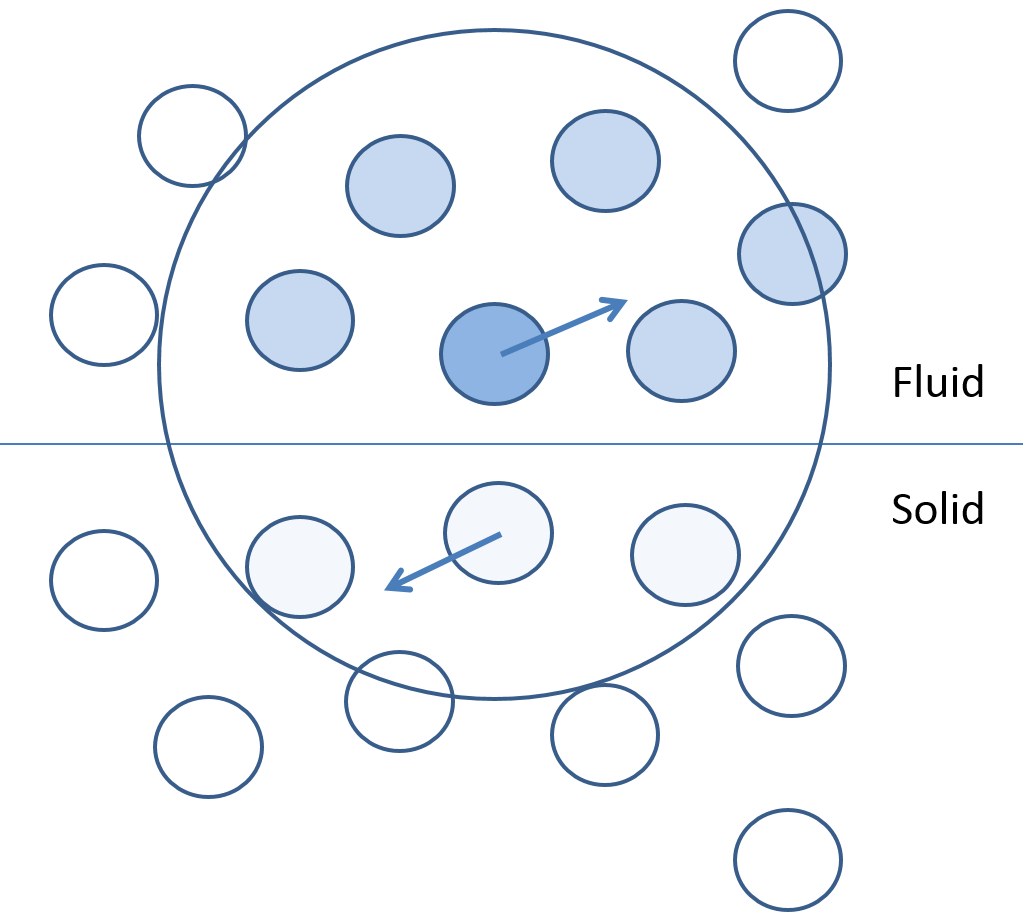
\includegraphics[width=0.45\linewidth]{Figures/3.Chapter/Ghost_particles}
	\caption{Scheme of ghost particles boundary condition.}
	\label{fig:Ghost_particles} 
\end{figure}
%

Both particles have the same density, but opposite normal and tangential velocities. Two disadvantages arise with this approach: complex geometries are extremely difficult to model (sharp angles, thin plates, hollow boxes) and the number of particles in the system may vary at each time step, a further implementation complication, explored in Section \ref{cap:chapter_hpc}. 


Repulsive particles \citep{Monaghan-1999} represent stationary particles that do not respect the conservation equations, but instead apply \textit{ad-hoc} forces to approaching fluid particles. The forces may be based on Lennard-Jones potentials, and a series of interpolation procedures are carried out to assure the continuity of a force field perceived by a fluid particle moving in an arbitrary direction from the boundary, as represented in Figure \ref{fig:repulsive_particles}.
%
\begin{figure}[H]
	\centering
	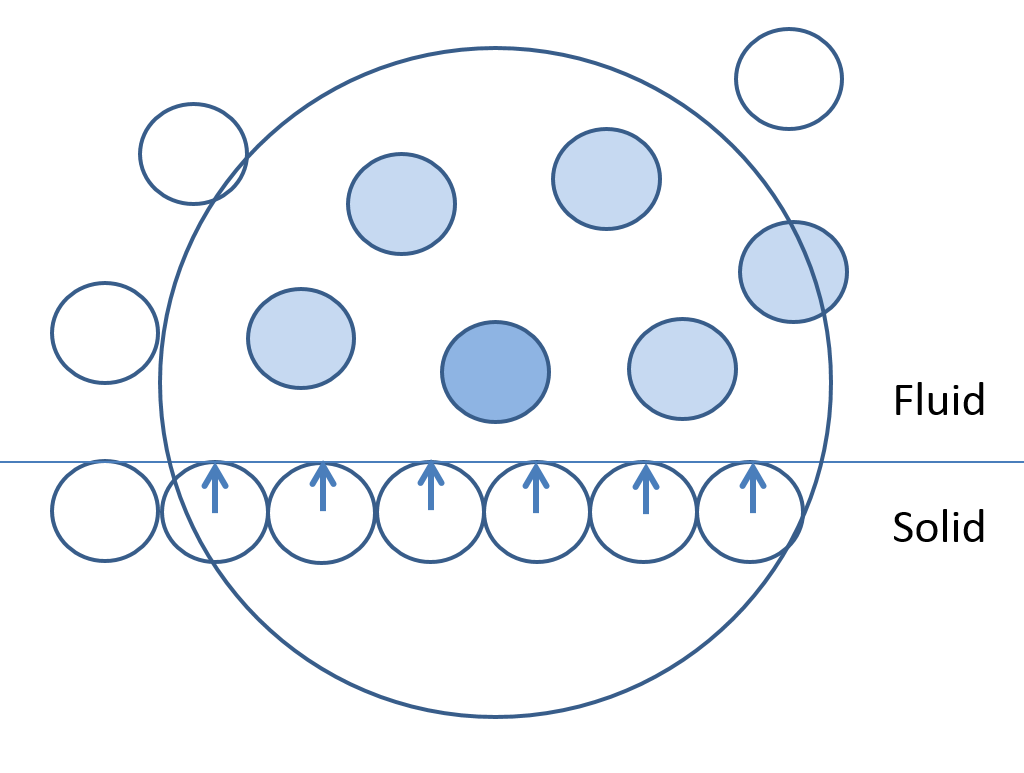
\includegraphics[width=0.45\linewidth]{Figures/3.Chapter/Repulsive_particles}
	\caption{Scheme of repulsive particles boundary condition.}
	\label{fig:repulsive_particles} 
\end{figure}
%

Dynamic particles were introduced by \cite{Dalrymple-2000} and further studied by \cite{Crespo-2007}, that devised them as fluid particles with an externally imposed motion. The particles respect Equations \eqref{eq:sph_navier_cont} and \eqref{eq:sph_navier_momentum_I} but their position is not given by integrating the velocity in time. A static boundary will have zero velocity (traditional arrangement in Figure \ref{fig:Dynamic_particles}) and a moving boundary will have a prescribed motion.
%
\begin{figure}[H]
	\centering
	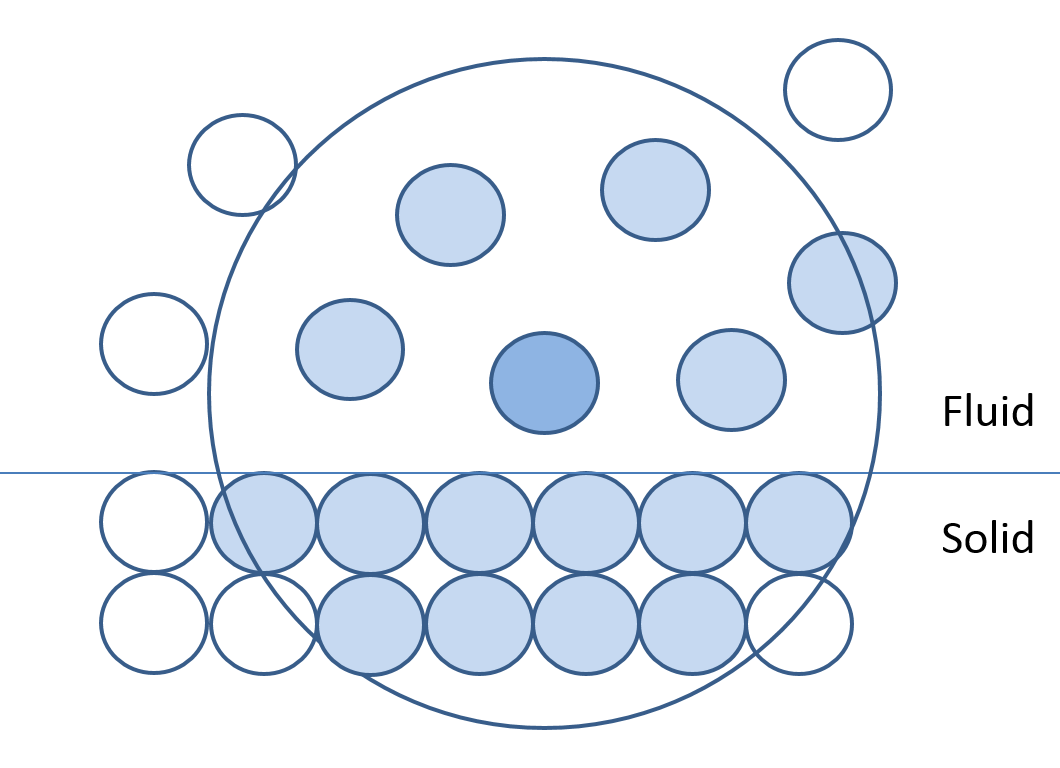
\includegraphics[width=0.45\linewidth]{Figures/3.Chapter/Dynamic_particles}
	\caption{Scheme of dynamic particles boundary condition.}
	\label{fig:Dynamic_particles} 
\end{figure}
%

A known difficulty of this formulation is the overestimation of the density \citep{Price-2008,Saitoh-2013}, resulting from an entropy jump across the fluid/solid interface. This results in an increased distance of fluid-solid particles due to the added force from the pressure gradient, effectively disturbing the viscous forces computed at that interface \citep{Colagrossi-2003}.

Boundary integral ideas are being explored in order to complete the kernel around boundaries, namely, analytically summing the missing terms. The boundary integral conditions \citep{Ferrand-al-2013, Mayrhofer-al-2015} are promising but still face many challenges related to complex geometries and efficient implementations.

This work will employ dynamic boundary conditions throughout, due to the simplicity and potential of the implementation. The solid body discretization presented in Section \ref{sec:solid-discretization} will also use the same framework.




\newpage
\section{Solid discretization: combining SPH and DEM}
\label{sec:solid-discretization}

The purpose of this Section is to devise a framework where the dynamics of solid bodies of arbitrary shape can be discretized in a way that solid-fluid interactions become trivial in the context of the fluid discretization presented in Section \ref{sec:fluid-discretization}. Section \ref{sec:solid-discretization_body} presents that general framework, where discrete equations for rigid body dynamics are introduced, generalizing the source of accelerations affecting a body. 

The \ac{DEM} model is introduced in Section \ref{sec:solid-discretization_force}, where the particular case of solid-solid interaction is explored. Traditional \ac{DEM} models are analyzed, as well as their numerical properties.

The result of this section is a \ac{DCDEM}, fully respecting the requirements of an accurate and robust model for the treatment of solid bodies with 6 \ac{DOF} in a multiphase setting.


\subsection{Rigid body discretization}
\label{sec:solid-discretization_body}

In the domain frame reference, the equations for a rigid body $I$ can be written as
%
\begin{equation} \label{eq:rigid_linear_newton}
	M_I\frac{d\ve{V}_I}{dt}=\sum_i \ve{F_i}
\end{equation}

\begin{equation} \label{eq:rigid_angular_newton}
	\ve{I}_I\frac{d\ve{\Omega}_I}{dt}=\sum_i(\ve{r}_i-\ve{R}_I)\times \ve{F_i},
\end{equation}
%
where body $I$ possesses a mass $M_I$, velocity $\boldsymbol{V}_I$, inertial tensor $\boldsymbol{I}_I$, angular velocity $\boldsymbol{\Omega}_I$ and center of gravity $\boldsymbol{R}_I$, and is subjected to an arbitrary number of forces $\ve{F_i}$, applied at points $\ve{r_i}$. 

In a particulate method it is trivial to idealize sub sets of particles in the domain whose variables are integrated in time with a different set of equations. If one uses Newton's equations for rigid body dynamics, then, that system of particles represents a rigid body. If body $I$ is a collection of particles\footnote{In this section $I$ is used for both the index of the rigid body in question and as the set of indexes from the particles that constitute the body. The abuse of notation is employed since in this context, they are semantically coincident.}, then the right side of Equations \eqref{eq:rigid_linear_newton} and \eqref{eq:rigid_angular_newton} can easily be discretized by

%
\begin{equation} \label{eq:rigid_linear}
	M_I\frac{d\ve{V}_I}{dt}=\sum_{k\in I} m_k \frac{{d{\ve{u}_k}}}{{dt}}
\end{equation}
%
\begin{equation} \label{eq:rigid_angular}
	\ve{I}_I\frac{d\ve{\Omega}_I}{dt}=\sum_{k\in I}m_k(\ve{r}_k-\ve{R}_I)\times \frac{{d{\ve{v}_k}}}{{dt}}
\end{equation}
%
$m_k {{d{\boldsymbol{u}_k}}}/{{dt}}$ represents the force by unit mass applied to particle $k$, belonging to body $I$. This force encompasses body forces (gravity), fluid resultants as well as the result of any rigid contact that might occur. This is inline with the work of \cite{Koshizuka-1998}, that first applied this idea in the context of \ac{MPS}.

Expressions \eqref{eq:rigid_linear} and \eqref{eq:rigid_angular} are obtained directly from applying \eqref{eq:rigid_linear_newton} and \eqref{eq:rigid_angular_newton} to a system of particles, i.e., they inherently conserve linear and angular momentum, as they are simple conservation laws. This is an advantage of particulate Lagrangian discretizations, since they are an exact representation of particle systems if the closure terms are also exact. For this system, it is simple to write the center of mass $\ve{R}_I$ and inertia tensor $\ve{I}_I$

%
\begin{equation} \label{eq:rigid_center_inertia}
	\ve{R}_I=\frac{1}{n_I}\sum_{k\in I} \ve{R}_k; \;\;\;\;\;\;\; \ve{I}_I=\sum_{k\in I}=m_k[\ve{r}_k-\ve{R}_I][\ve{r}_k-\ve{R}_I]
\end{equation}
%
where $n_I$ is them number of particles that constitute body $I$, $[\ve{r}_k-\ve{R}_I]$ is the skew-symmetric matrix built from $\ve{r}_k-\ve{R}_I$. Keeping in the domain frame reference implies that these quantities need to be recomputed whenever the system suffers an acceleration. 

Forces resulting from solid-fluid interaction are computed with Equation \eqref{eq:sph_navier_momentum_I}, where the viscous formulation provides a viscous drag closure. No \textit{ad-hoc} terms are added, since all the dynamics are a result of the fundamental, particle-wise, solution of Equations \eqref{eq:rigid_linear} and \eqref{eq:rigid_angular}.

This formulation can be seen as an extension of the dynamic boundary conditions introduced in Section \ref{sec:BCs}. As such, it suffers from the same overestimation of the density across the fluid/solid interface \cite{Price-2008,Saitoh-2013}, resulting from an entropy jump. The inclusion of the $\delta$-SPH diffusive term in Equation \eqref{eq:sph_navier_cont_delta_sph} allows for an apparently correct density estimation across the interface, as explored in the Results Section. The particles belonging to body $I$ are then moved according to

%
\begin{equation} \label{eq:rigid_propag_vel}
	\ve{u}_k= \ve{V}_I+\ve{\Omega}_I \times (\ve{r}_k-\ve{R}_I),
\end{equation}
%
\textit{i.e.}, the velocity given by propagating the rigid body velocities.


\subsection{Force discretization: the DEM model}
\label{sec:solid-discretization_force}

Forces $m_k {{d{\boldsymbol{u}_k}}}/{{dt}}$ will rise whenever a particle interacts with another. In the particular case of a solid-solid collision, the contact force is decomposed into $\ve{F}_n$ and $\ve{F}_t$, normal and tangential components respectively. Both of these forces will take forms explored in Section \ref{sec:solid_model}, with the addition of viscous dissipation effects. This is because two colliding bodies undergo a deformation which will be somewhere between perfectly inelastic and perfectly elastic, usually quantified by the normal restitution coefficient

%
\begin{equation} \label{eq:rest_coeff_def}
	e_n=-\frac{v_n|_{t=t^n}}{v_n|_{t=0}}, \;\;\;\; e\in[0,1]
\end{equation}
%
where $t=t^n$ is the instant at the end of collision and $t=0$ is the instant immediately before.

Forces are further decomposed into a repulsion force, $\boldsymbol{F}^r$, arising from the elastic deformation of the material, and a damping force, $\boldsymbol{F}^d$, for the viscous dissipation of energy during the deformation. Other dissipative mechanisms, such as plastic deformation and emission of elastic waves, excited from impact, will not be considered. The elastic waves are always present, but carry very little energy \citep{Shaefer-1996}, and are usually disregarded. Plastic deformation is not considered directly as its effects can, to some extent, be included in the viscous dissipation terms.

Figure \ref{fig:dem_scheme} generally illustrates the proposed viscoelastic DEM mechanism between two interacting particles.

%
\begin{figure}[ht!]
	\centering
	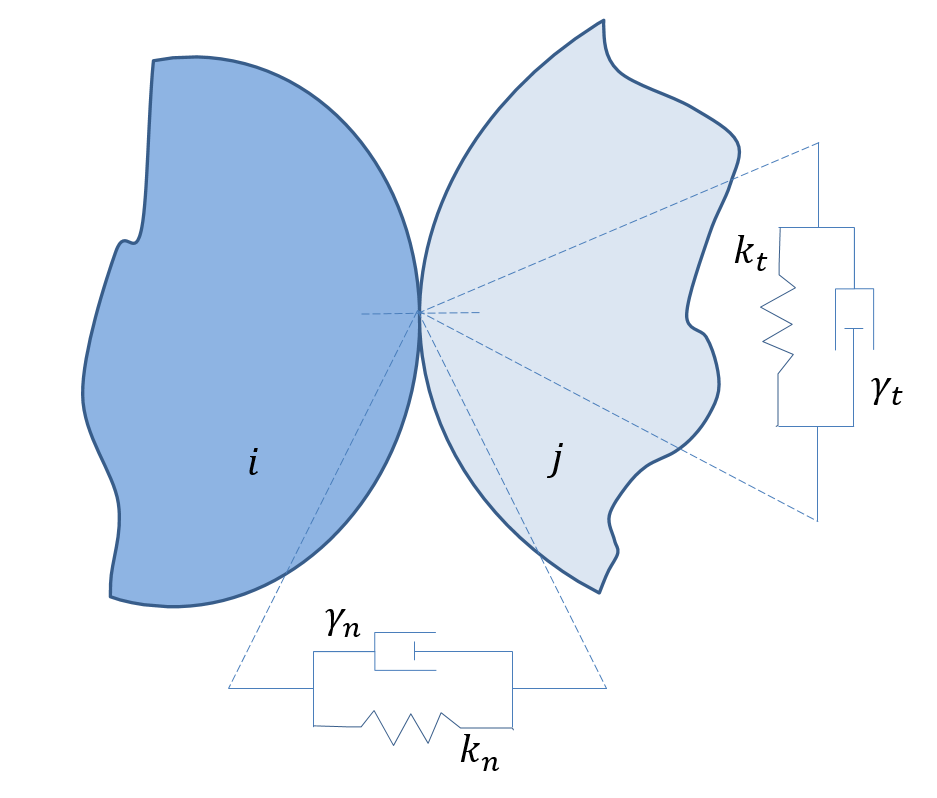
\includegraphics[width=0.60\linewidth]{Figures/3.Chapter/DEM_contacts}
	\caption{Scheme of DEM mechanism.}
	\label{fig:dem_scheme} 
\end{figure}
%
Every interaction is conceptualized as a system of springs and dampers. A general expression for the normal force in such viscoelastic model will be

%
\begin{equation} \label{eq:normal_viscoelastic_I}
	\ve{F}_{n,ij}=\ve{F}_n^r+\ve{F}_n^d=k_{n,ij}\delta_{ij}^{p_1}\ve{e}_{ij}-\gamma_{n,ij}\delta_{ij}^{p_2}\dot{\delta}_{ij}\ve{e}_{ij},
\end{equation}
%
where $k_{n,ij}$ is the normal stiffness constant of pair $ij$, $\delta_{ij}=\max(0, (d_i+d_j)/2-|\ve{r_{ij}}|)$ is the particle overlap, $\ve{e}_{ij}$ is the unit vector between the two mass centers and $\gamma_{n,ij}$ is the normal damping constant. For $p_1=p_2=1$, the mechanism is linear, corresponding to a simple damped harmonic resonator. An analytical solution \citep{Shaefer-1996} shows that this leads to a constant normal restitution coefficient, independent of the impact velocity

%
\begin{equation} \label{eq:linear_restitution_coeff}
	e_{n,ij}=\exp\left( -\frac{\gamma_{n,ij}}{2M^*}t_{c,ij} \right)
\end{equation}
%
where $M^*={m_im_j}/({m_i+m_j})$ and $t_{c,ij}$ is the contact duration, given by

%
\begin{equation} \label{eq:linear_tc}
	t_{c,ij}=\pi \left( \frac{k_{n,ij}}{M^*}- \left( \frac{\gamma_{n,ij}}{2M^*} \right)^2 \right)^{-1/2}
\end{equation}
%
Experimental studies using pendulum devices indicate that the $e_n$ and $t_c$ should depend on impact velocity however. Figures \ref{fig:Restitution_coeff} and \ref{fig:t_c_exp} both compiled by \cite{Kruggel-Emden-2007}, show that dramatic variations of these quantities may be registered.

%
\begin{figure}[ht!]
	\centering
	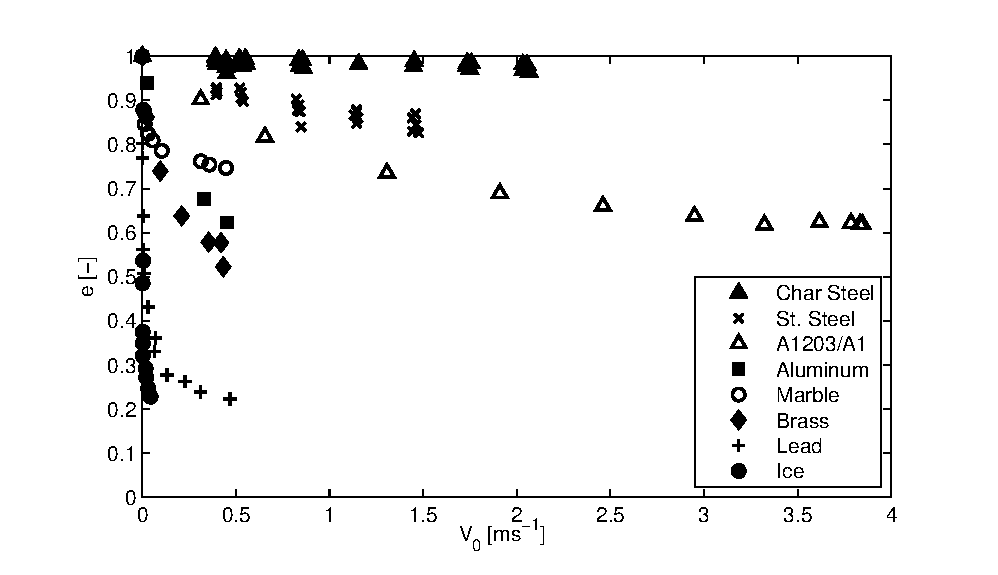
\includegraphics[width=0.73\linewidth]{Figures/3.Chapter/e_vo}
	\caption{Restitution coefficient $e$ as a function of initial normal velocity $V_0$ \citep{Kruggel-Emden-2007}.}
	\label{fig:Restitution_coeff} 
\end{figure}
%

%
%\begin{figure}[ht!]
%	\centering
%	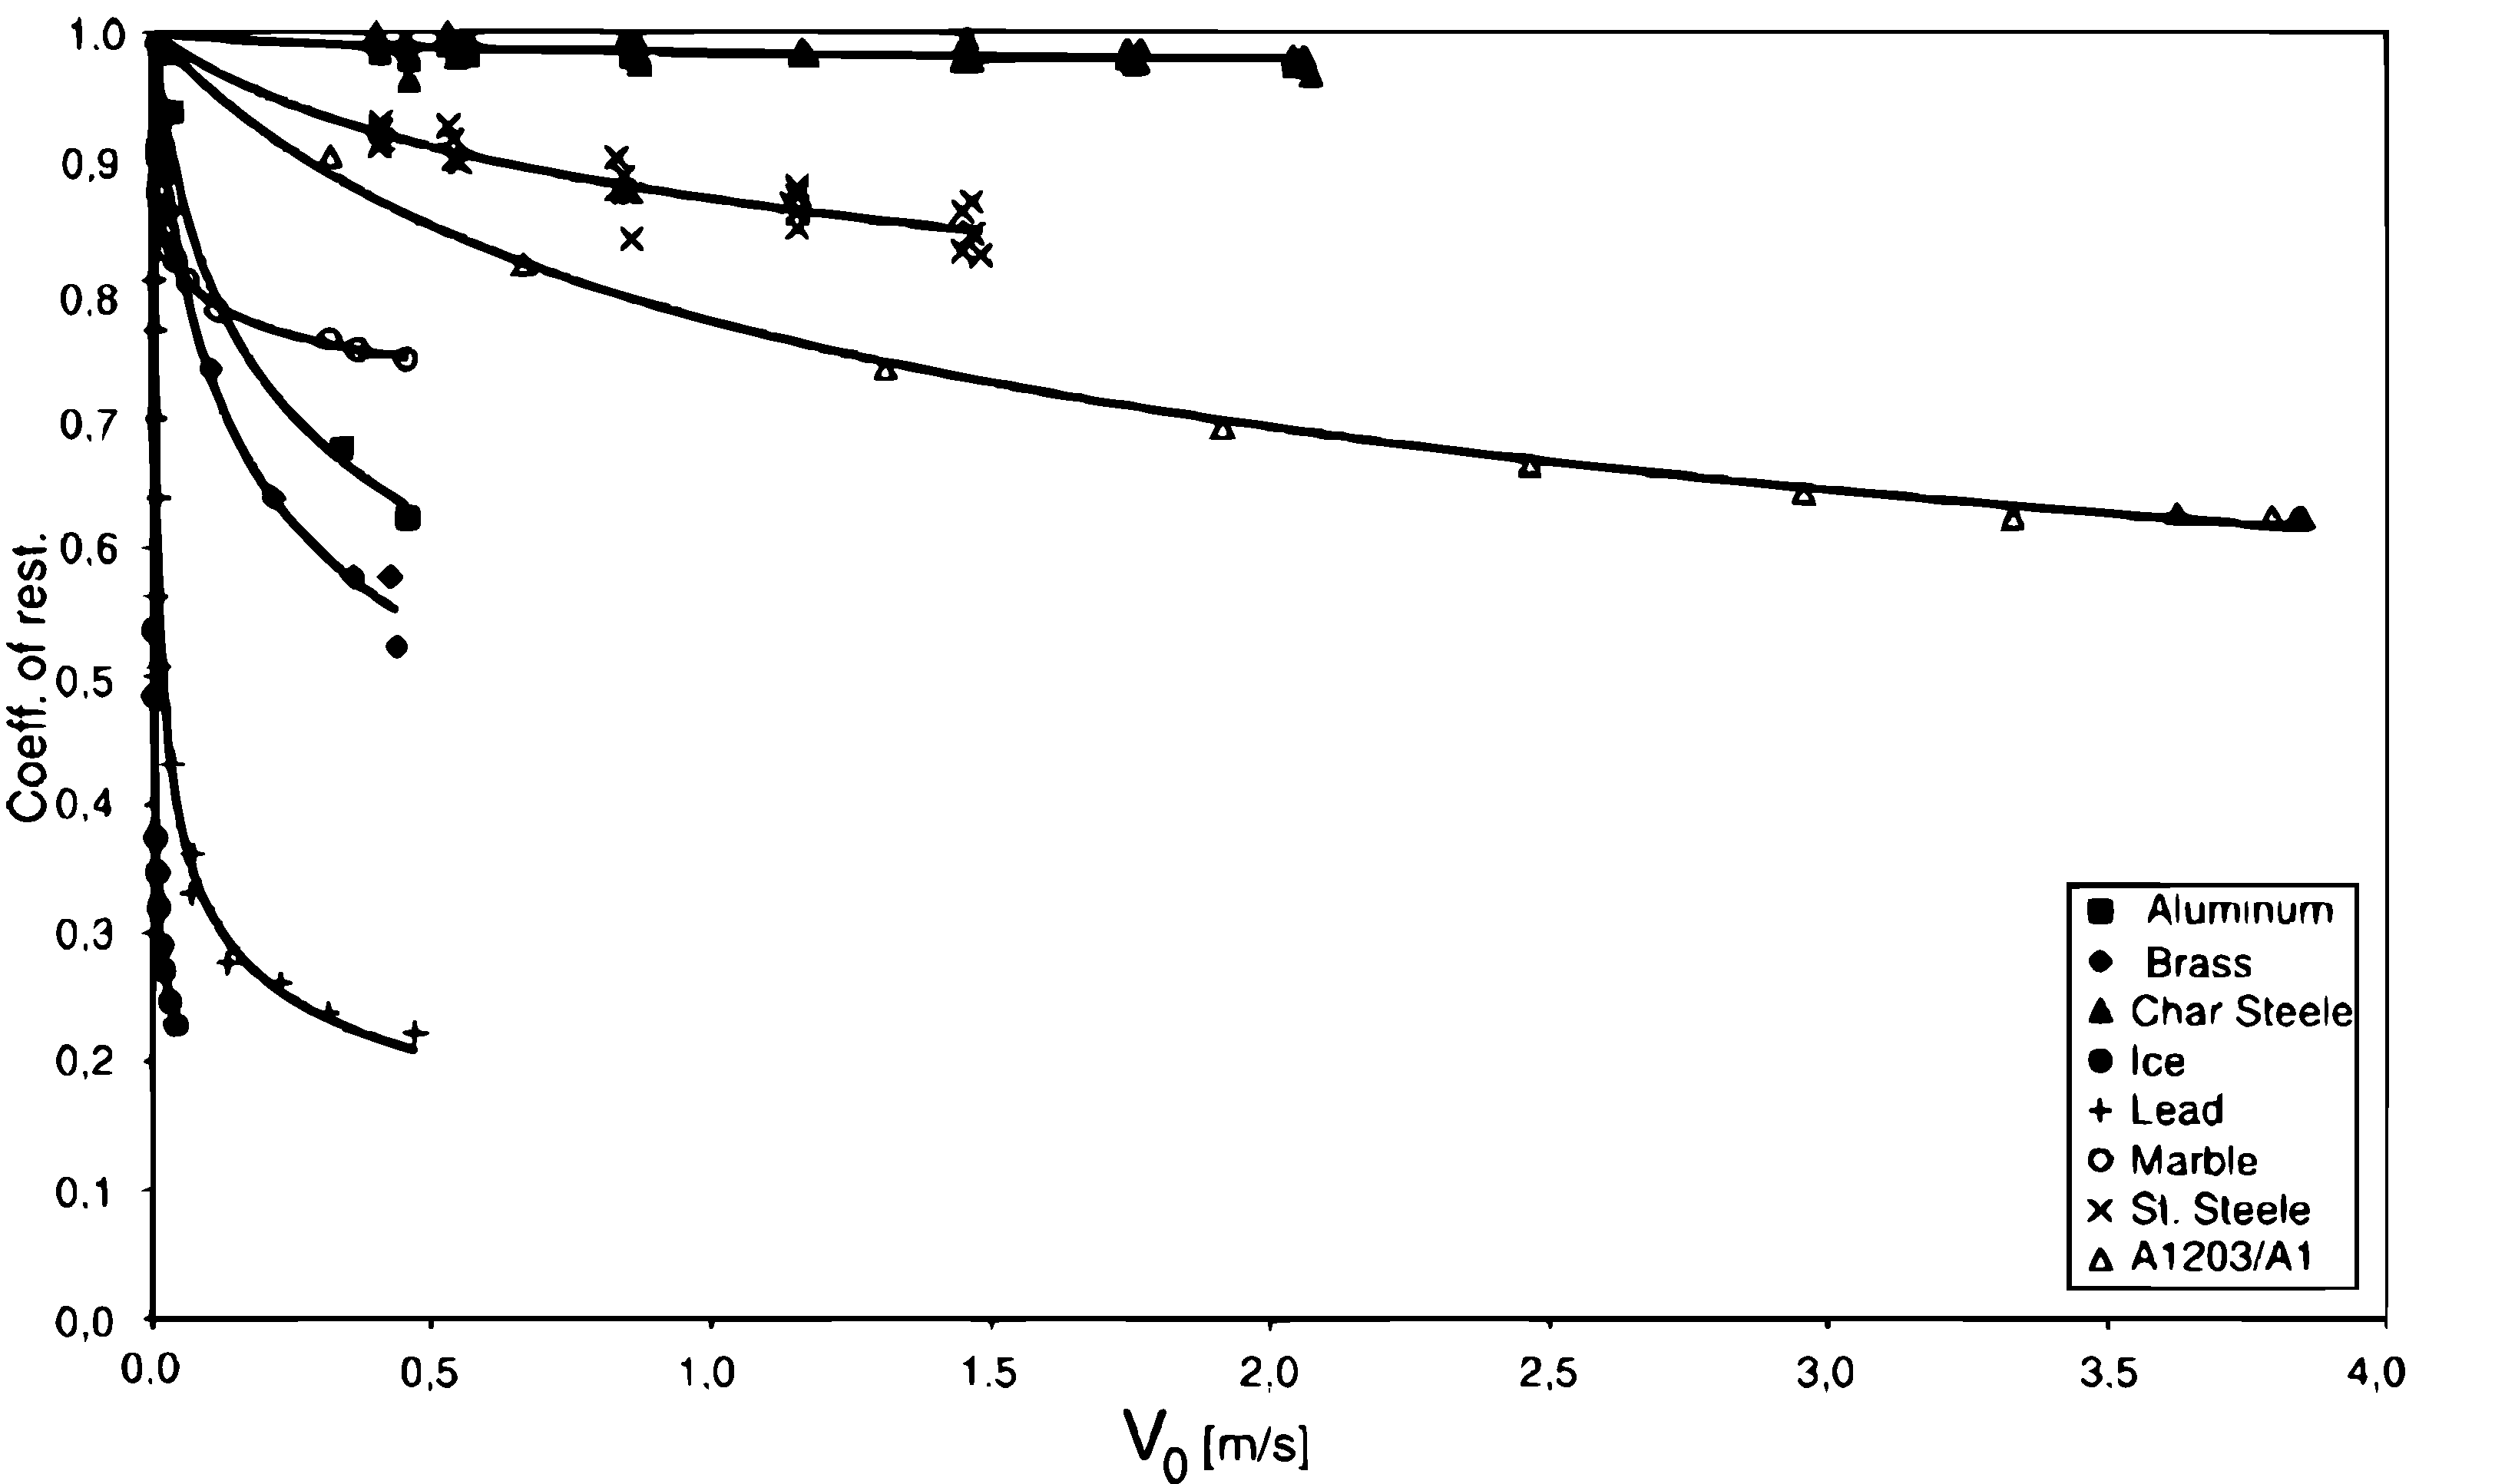
\includegraphics[width=0.80\linewidth]{Figures/3.Chapter/rest_coeff_exp}
%	\caption{Restitution coefficient $e$ as a function of impact normal velocity $V_0$ \citep{Kruggel-Emden-2007}.}
%	\label{fig:Restitution_coeff} 
%\end{figure}
%
%
\begin{figure}[ht!]
	\centering
	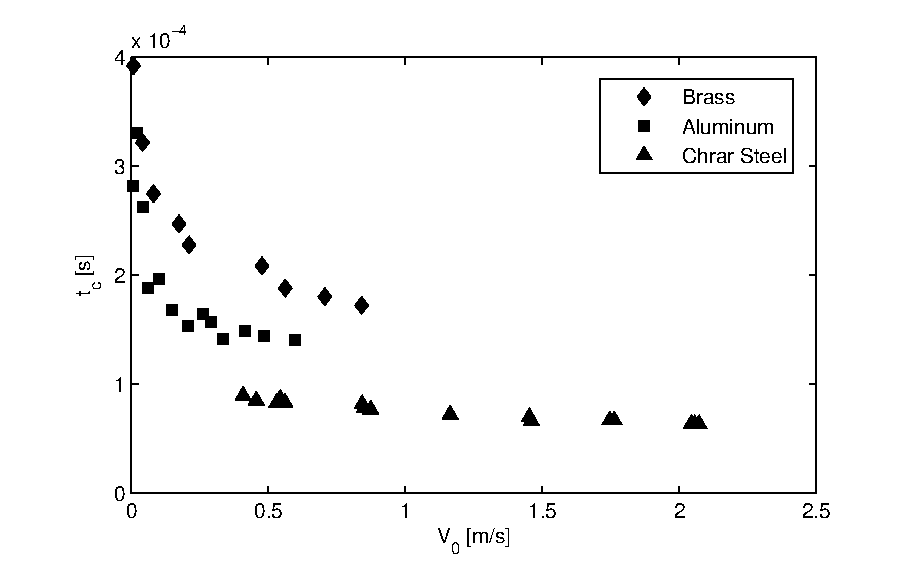
\includegraphics[width=0.70\linewidth]{Figures/3.Chapter/tc_vo}
	\caption{Duration of contact $t_c$ as a function of the impact normal velocity $V_0$ \citep{Kruggel-Emden-2007}.}
	\label{fig:t_c_exp} 
\end{figure}
%
%
%\begin{figure}[ht!]
%	\centering
%	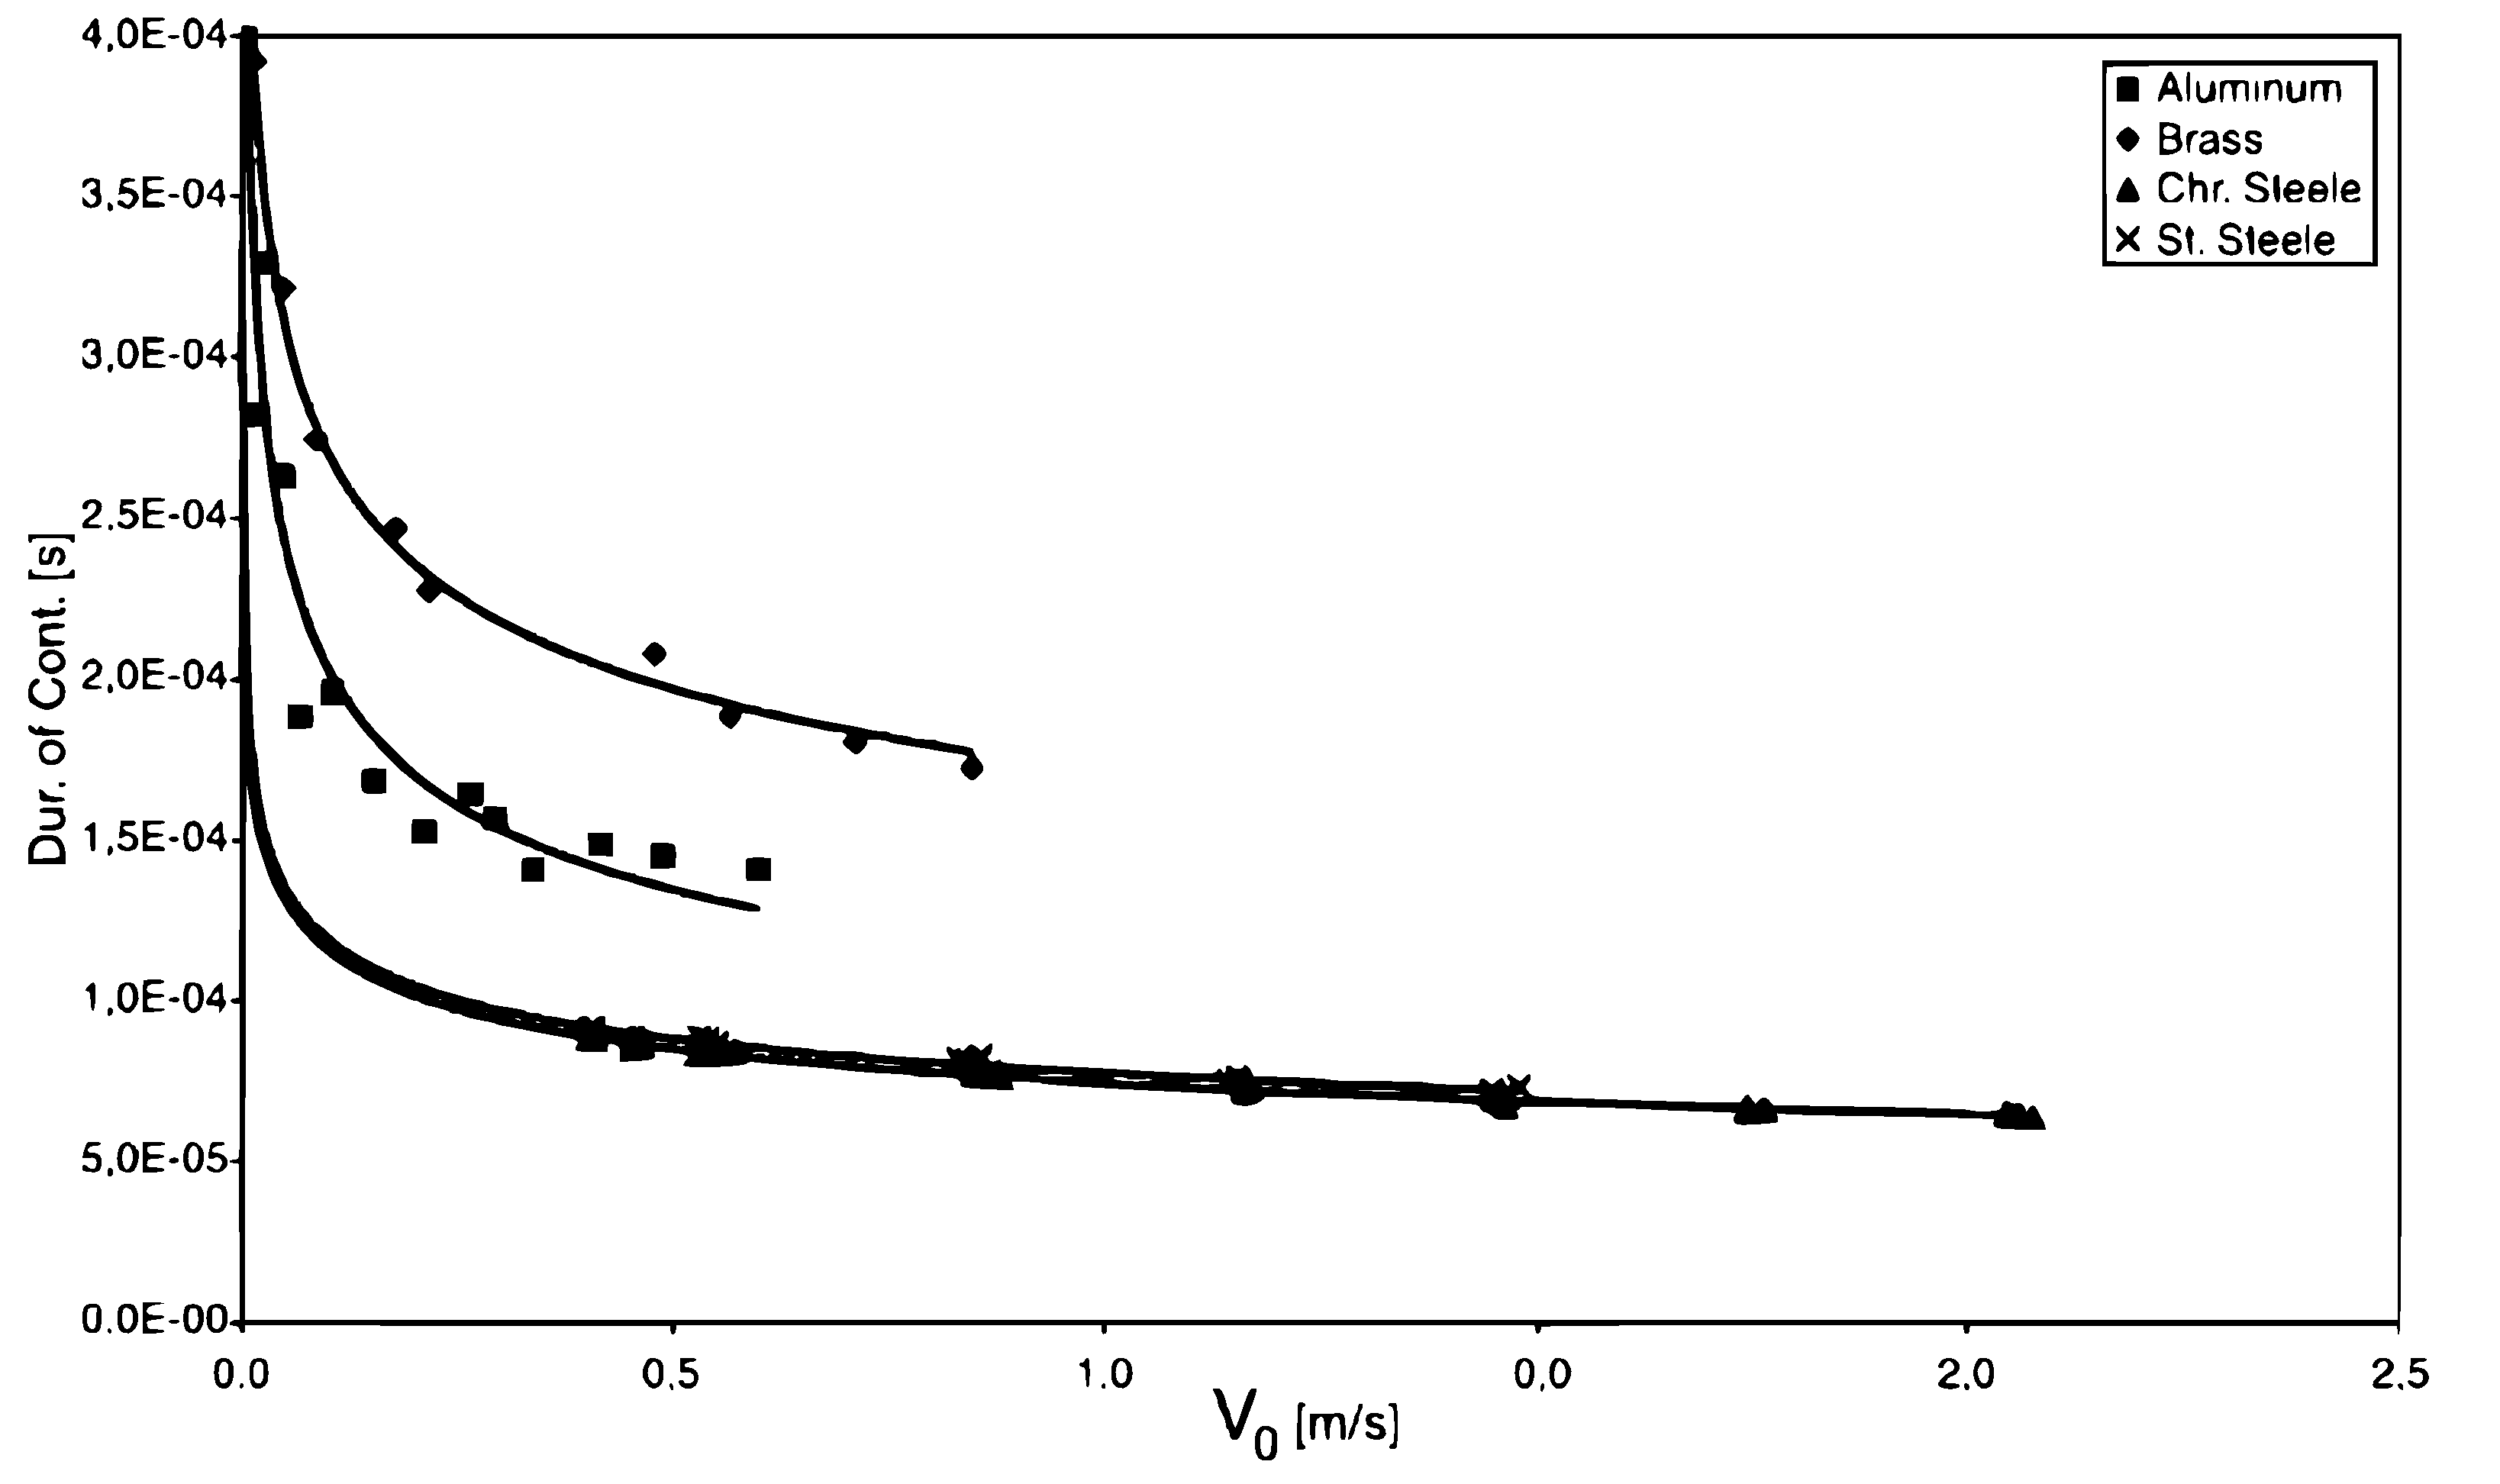
\includegraphics[width=0.80\linewidth]{Figures/3.Chapter/impact_time}
%	\caption{Duration of contact $t_c$ as a function of the impact normal velocity $V_0$ \citep{Kruggel-Emden-2007}.}
%	\label{fig:t_c_exp} 
%\end{figure}
%

Non-linear models allow to overcome the limitation imposed by a constant restitution coefficient and contact duration. \cite{Kuwabara-1987}, \cite{Brilliantov-1996} and \cite{Brilliantov-2001} proposed a fully non-linear model that reads

\begin{equation} \label{eq:non_linear_hertz_normal}
	\ve{F}_{n,ij}=\ve{F}_n^r+\ve{F}_n^d=k_{n,ij}\delta_{ij}^{3/2}\ve{e}_{ij}-\gamma_{n,ij}\delta_{ij}^{1/2}\dot{\delta}_{ij}\ve{e}_{ij},
\end{equation}
%
The stiffness, recovering the elastic Hertz model from Section \ref{sec:solid_model}, is given by a form of Equation \eqref{eq:hertz_III} 

%
\begin{equation} \label{eq:rigidity_hertz}
	k_{n,ij}=\frac{4}{3}E^*\sqrt{R^*}
\end{equation}
%
Considering exclusively the repulsive part of Equation \eqref{eq:non_linear_hertz_normal}, \cite{Shaefer-1996} notes that $t_{c,ij}$ is no longer independent from the normal velocity impact $v_{n,ij}$

%
\begin{equation} \label{eq:non_linear_tc}
	t_{c,ij}=3.21 \left( -\frac{M^*}{k_{n,ij}} \right)^{2/5}v_{n,ij}^{-1/5}
\end{equation}
%
implying that there is no longer an intrinsic time scale to collisions, as expected from experimental data.

\cite{Brilliantov-1996} and \cite{Brilliantov-2001} proposed that the viscous damper coefficient $\gamma_{n,ij}$ is a material property, obtainable from the bulk viscosities of the materials in collision and the local curvature at impact point. However, very little studies have been devoted to bulk viscosities and as a consequence $\gamma_{n,ij}$ is traditionally treated as a calibration parameter. \cite{Cummins-2011} writes an expression for $\gamma_{n,ij}$ depending exclusively on a normal restitution coefficient

%
\begin{equation} \label{eq:gamma_dem}
	\gamma_{n,ij}=-\frac{\log{e_{n,ij}}}{\sqrt{\pi^2+\log^2{e_{n,ij}}}}
\end{equation}
%
Expression \eqref{eq:gamma_dem} used in the context of a non-linear model, is ambiguous. In practice, a constant value for $e_{n,ij}$ will be used to compute $\gamma_{n,ij}$, that will lead to a non-constant, effective $e_{n,ij}$, depending on the impact velocity.

Figure \ref{fig:e_hertz} shows $e_{n,ij}$ as a function of $v_{n,ij}$, for the linear model and for the non-linear Hertz model (Expression \eqref{eq:non_linear_hertz_normal})

%
\begin{figure}[ht!]
	\centering
	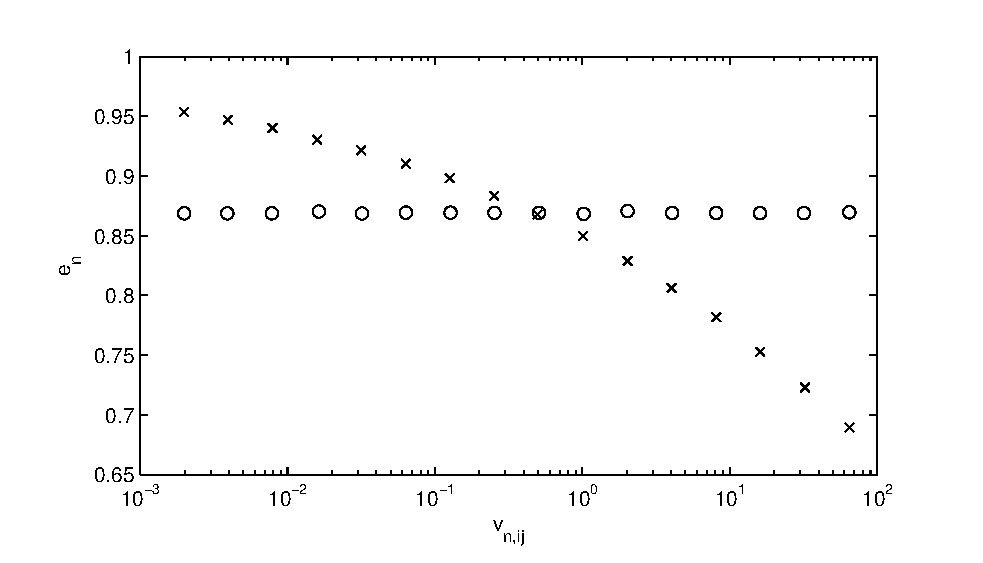
\includegraphics[width=0.80\linewidth]{Figures/3.Chapter/e_hertz}
	\caption{Normal restitution coefficient $e_{n,ij}$ as a function of the impact normal velocity $v_{n,ij}$. Linear force ($\circ$), Non-linear Hertz ($\times$)}
	\label{fig:e_hertz} 
\end{figure}
%
For the linear case $k_n=7.32\times10^6$ Nm$^{-1}$ and $\gamma_n=2.06$ kg s$^{-1}$, resulting in $e_n=0.87$. For the non-linear model, $\gamma_n=190$ m$^{-1/2}$s$^{-1}$, in order to produce comparable $e_n$ in the selected $v_{n,ij}$ range. As expected, the linear model produces a constant $e_n$. Force \eqref{eq:non_linear_hertz_normal} leads to an inversely proportional $e_{n,ij}$ with $v_{n,ij}$, i.e., $(1-e_{n,ij})\sim v_{n,ij}^{1/5}$, in agreement with experimental results (Figure \ref{fig:Restitution_coeff}).


Regarding tangential contacts, friction is modeled using the same model, as indicated in Figure \ref{fig:dem_scheme}. The mechanism can be reproduced by a linear dash-pot 

%
\begin{equation} \label{eq:elastic_fric}
	\ve{F}_{t,ij}=\ve{F}_t^r+\ve{F}_t^d=k_{t,ij}\delta^t_{ij}\ve{e}^t_{ij}-\gamma_{t,ij}\dot{\delta}^t_{ij}\ve{e}^t_{ij}
\end{equation}
%
where the stiffness and damping constants are derived to be

%
\begin{equation} \label{eq:fric_coeffs}
	k_{t,ij}=2/7k_{n,ij}; \;\;\;\;\; \gamma_{t,ij}=2/7\gamma_{n,ij},
\end{equation}
%
as to insure internal consistency of the time scales required for stability \citep{Hoomans-2000}. This mechanism models the static and dynamic friction mechanisms by a penalty method. The body does not statically stick at the point of contact, but is constrained by the spring-damper system. This force must be bounded above by the Coulomb friction law introduced by Equation \eqref{eq:coulomb_friction}. The Coulomb law is modified with a sigmoidal function in order to make it continuous around the origin regarding the tangential velocity \citep{Vetsch-2011}:

%
\begin{equation} \label{eq:fric_I}
	\ve{F}_{t,ij}=\min(\mu_{fIJ} \ve{F}_{n,ij} \tanh (8\dot{\delta}^t_{ij})\ve{e}^t_{ij};\;\; \ve{F}_{t,ij}),
\end{equation}
%
\noindent where $\mu_{fIJ}$ is the friction coefficient at the contact of $I$ and $J$ and is simply taken as the average of the two friction coefficients of the distinct materials.
\section{Time Integration and Stability Region}
\label{sec:dt}

The ordinary differential equations described in Sections \ref{sec:fluid-discretization} and \ref{sec:solid-discretization} may be integrated in time using a stable method. Traditionally Symplectic schemes are preferred in Hamiltonian systems due to the time-reversibility in the absence of dissipative terms, as well as implicit conservation properties \citep{Monaghan-2005}, leading to a lesser energy drift in long computations. Both \ac{SPH} and \ac{DEM} methods use the Symplectic scheme due to these characteristics. An explicit second-order with time accuracy of $O(dt^2)$ Symplectic integrator is used, using two half-steps with a predictor-corrector strategy:

%
\begin{equation} \label{eq:symplectic_predictor}
	Q_i^{n+1/2}= Q_i^{n}+\frac{1}{2}\Delta t \frac{dQ_i^{n}}{dt}
\end{equation}
%
where $Q$ takes the form of $\rho$, $\ve{r}$ or $\ve{u}$, to integrate for density, position and velocity, respectively. For the corrector step

%
\begin{equation} \label{eq:symplectic_predictor_II}
	Q_i^{n+1}= Q_i^{n+1/2}+\frac{1}{2}\Delta t \frac{dQ_i^{n+1/2}}{dt}
\end{equation}
%
where the corrected velocity $\ve{u}_i^{n+1}$ is used to update the corrected position $\ve{r}_i^{n+1}$ and both are used to compute the corrected density $\rho_i^{n+1}$.

The stability region of numerical schemes is traditionally assessed with a \ac{CFL} condition. This condition relates the length of the time step to a function of the spatial discretization and the maximum speed with which information can travel in the physical space. In the \ac{WCSPH} scheme, this translates to

%
\begin{equation} \label{eq:sph_stability_region_I}
\begin{split}
	\Delta t_1 = C \min_i \left( \frac{h}{C_s} \right)
\end{split}
\end{equation}
%
where $C$ is the \ac{CFL} parameter. For traditional explicit schemes $C\in[0;1]$. \cite{Monaghan-1989} recognized the diffusive nature of the artificial viscosity formulation (Equation \ref{eq:sph_artificial_visc_I}) and added the diffusive signal to the velocity signal, resulting in 
%
\begin{equation} \label{eq:sph_stability_region_II}
\begin{split}
	\Delta t_1 = C \min_i \left( \frac{h}{C_s + \max_j|\mu_{ij}|} \right)
\end{split}
\end{equation}
%

Another \ac{CFL} criterion can be derived by using particle accelerations \citep{Monaghan-1992}, ensuring that no particle penetration occurs:
%
\begin{equation} \label{eq:sph_stability_region_III}
	\Delta t_2 = C \min_i \left( \frac{h}{{|d\ve{u}_i/dt|}} \right)^{1/2}
\end{equation}
%

The stability region must also include the restrictions from the \ac{DEM} computations between two interacting solid particles, belonging to two different solids. Expression \eqref{eq:non_linear_tc} provides an estimate for the contact duration. \cite{Lemieux-2008}, \cite{Campbell-1985} and \cite{Brilliantov-2001} propose that fifty time steps is enough to resolve a contact without introducing significant errors in the force computation. As such, the \ac{DEM} criteria reads

%
\begin{equation} \label{eq:DEM_stability_region_I}
	\Delta t_3=\frac{t_{c,ij}}{50}=\frac{3.21}{50} \left( \frac{M^*}{k_{n,ij}} \right)^{2/5}v_{n,ij}^{-1/5}
\end{equation}
%
where $M^*$ is taken as the reduced mass of the rigid bodies, composed of several particles. The global time step can now be chosen as 
%
\begin{equation} \label{eq:sph_stability_region}
	\Delta t_ \leq C \min_i \left( \Delta t_1; \Delta t_2; \frac{\Delta t_3}{C} \right)
\end{equation}
%
